%
% main.tex -- Paper zum Thema <nerven>
%
% (c) 2020 Autor, OST Ostschweizer Fachhochschule
%
% !TEX root = ../../buch.tex
% !TEX encoding = UTF-8
%
\chapter{Nervenzellen\label{chapter:nerven}}
\kopflinks{Nervenzellen}
\begin{refsection}
\chapterauthor{Tobias Zuber und Dino Ramcilovic}
\section{Einleitung}

%\begin{itemize}
%\item
%Absätze werden gebildet, indem man eine Leerzeile einfügt.
%Die Verwendung von \verb+\\+ ist nur in Tabellen und Arrays gestattet.
%\item
%Die explizite Platzierung von Bildern ist nicht erlaubt, entsprechende
%Optionen werden gelöscht. 
%Verwenden Sie Labels und Verweise, um auf Bilder hinzuweisen.
%\item
%Beginnen Sie jeden Satz auf einer neuen Zeile. 
%Damit ermöglichen Sie dem Versionsverwaltungssysteme, Änderungen
%in verschiedenen Sätzen von verschiedenen Autoren ohne Konflikt 
%anzuwenden.
%\item 
%Bilden Sie auch für Formeln kurze Zeilen, einerseits der besseren
%Übersicht wegen, aber auch um GIT die Arbeit zu erleichtern.
%\end{itemize}

Die Informationsübertragung in unserem Körper wird vom Nervensystem übernommen.
Dies beinhaltet zum Beispiel das vermitteln von Reizen, welche die Augen oder Ohren aufgenommen haben,
an das Gehirn und das Senden von Befehlen vom Gehirn an die Muskeln.
Das Nervensystem besteht aus Nervernzellen, welche elektrische Signale generieren, von anderen Zellen aufnehmen und weiterleiten können.
Die Signale werden so von einer Zelle zur nächsten Zelle weitergeleitet, bis das Signal am Zielpunkt ist.
\subsection{Biologische Grundlagen}
In Abbildung \ref{fig:Aufbau Nervenzelle} ist der Aufbau einer Nervenzelle ersichtlich. 
\begin{figure}[H]
    \centering
    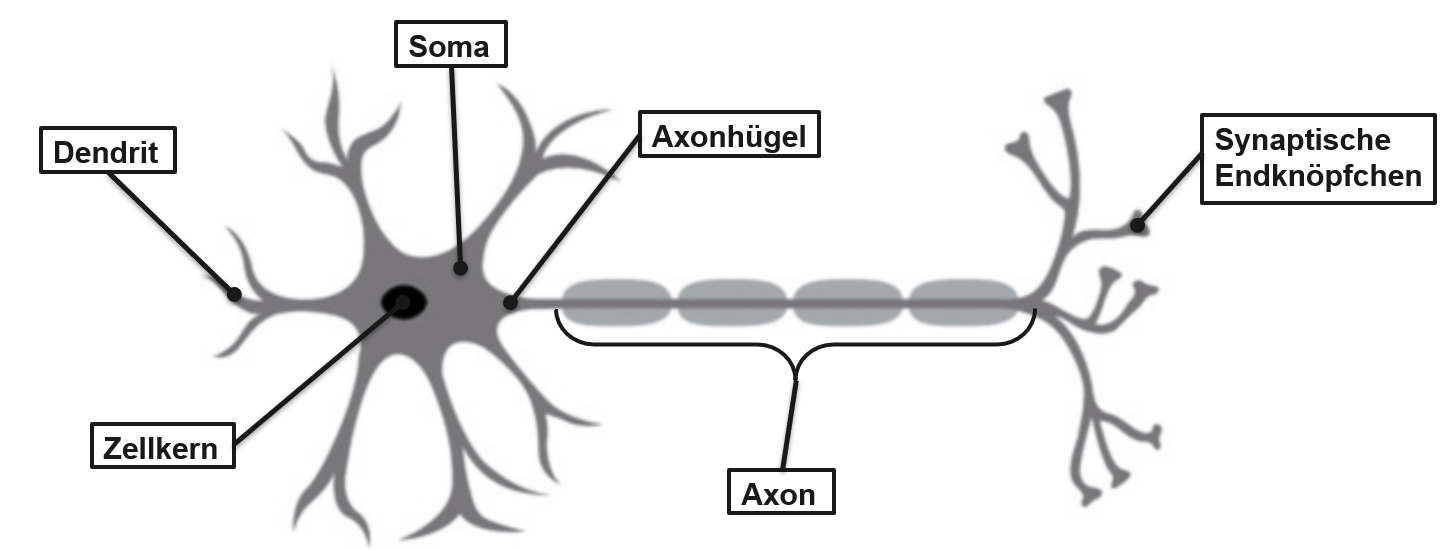
\includegraphics[width=\textwidth]{papers/nerven/Bilder/NervenAufbau2.png}
    \caption{Aufbau Nervenzelle}
    \label{fig:Aufbau Nervenzelle}
\end{figure}

\noindent
Dabei werden mit den Dendriten Signale empfangen. 
Im Axonhügel im Soma werden basierend auf den empfangenen Singalen elektrische Impulse erzeugt und mithilfe des Axons übertragen.
Die Synapsen sind mit der nächsten Zelle verknüpft und so wird das Signal immer weitergeleitet.

\subsection{Aktionspotential}
Die Nervenzelle besitzt für das Erzeugen von elektrischen Impulsen, das von den empfangenen Signalen bestimmt wird ein Interessantes Verhalten.
Um zu verhindern, dass im Axonhügel ungewollte elektrische Impulse entstehen, gibt es einen Spannungsschwellenwert,
den das empfangene Signal überschreiten muss.
Bei Signalen mit zu kleiner Spannung, wird dieses Signal sofort stark gedämpft und führt auch zu keinem elektrischen Impuls.
Wenn der Schwellenwert jedoch vom empfangenen Signal überschritten wird, gibt es sofort einen grossen elektrischen Impuls,
der entlang des Axons weitergeleitet wird. 
Diesen elektrischen Impuls nennt man Aktionspotential.
\begin{figure}[H]
    \centering
    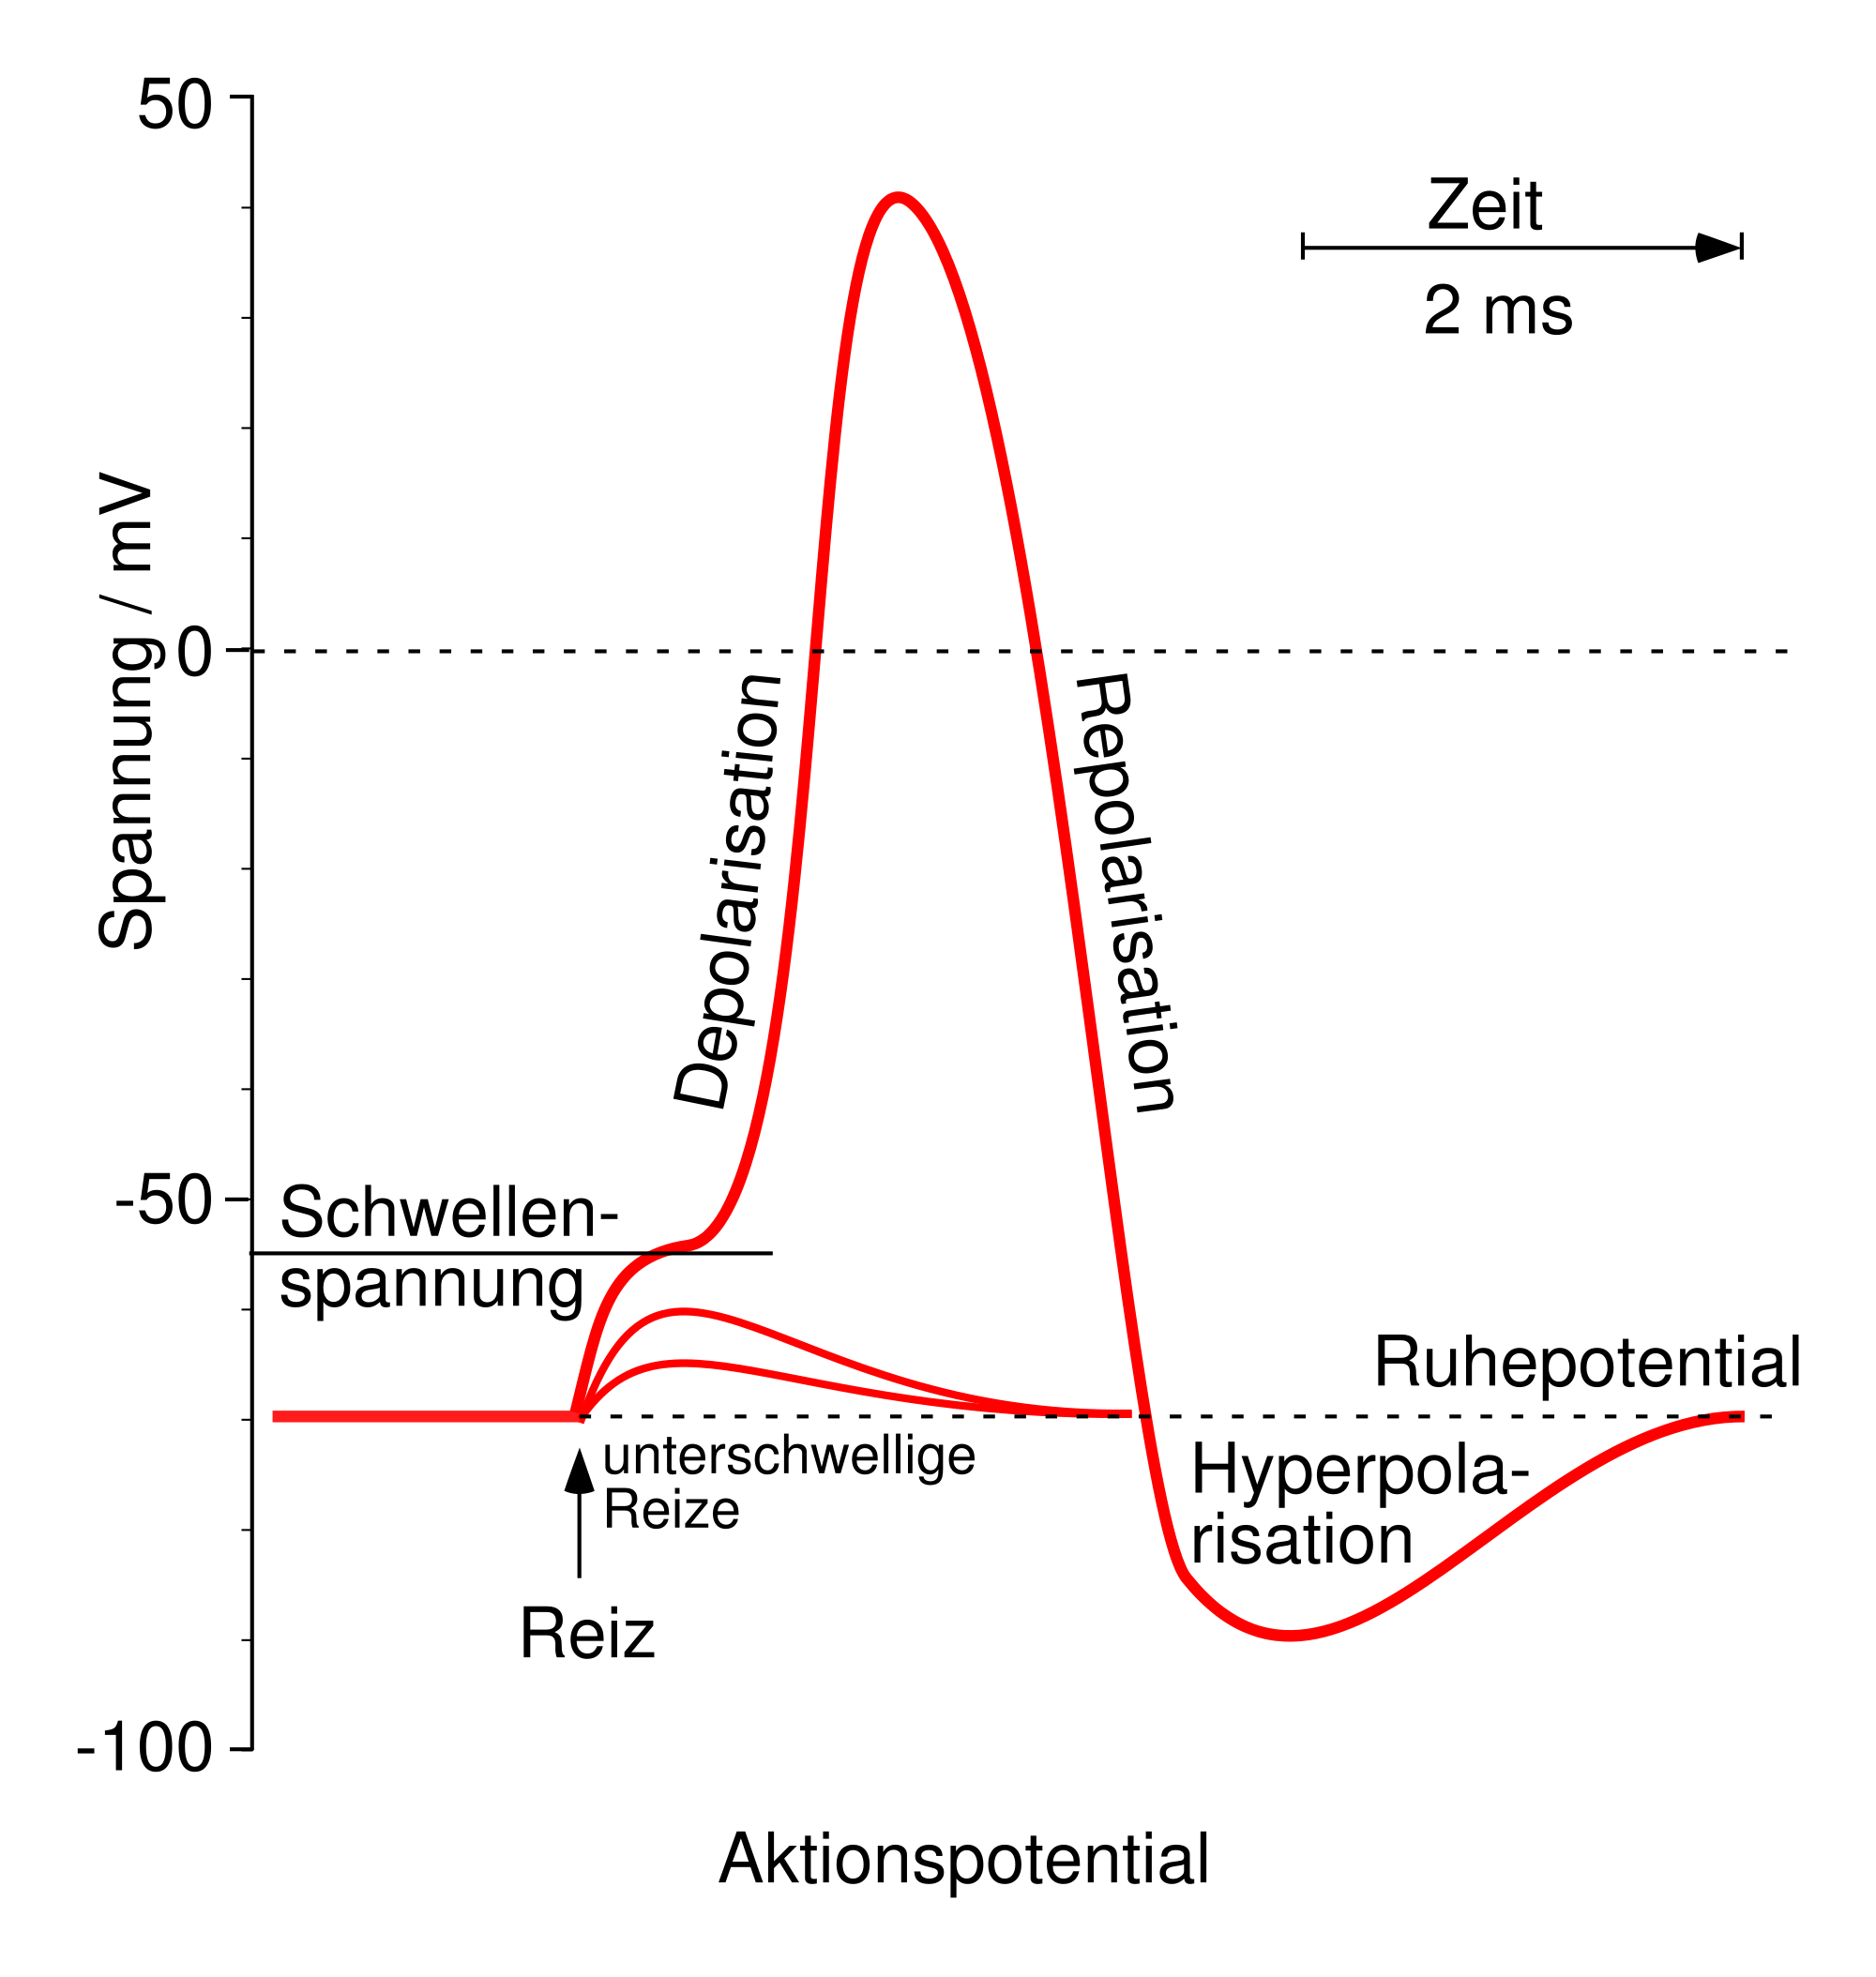
\includegraphics[width=0.9\textwidth]{papers/nerven/Bilder/Aktionspotential.png}
    \caption{Aktionspotential}
    \label{fig:Aktionspotential}
\end{figure}
\noindent
In Abbildung \ref{fig:Aktionspotential} ist ersichtlich wie ein Aktionspotential entsteht und schnell wieder abklingt.
Dabei besitzt diese Nervenzelle eine Ruhespannung von -70 Millivolt und einen Spannungsschwellenwert von -50 Millivolt.
Wenn die Nervenzelle einen Reiz, in Form eines elektrischen Signales erhält, wird eine Entscheidung getroffen. 
Ist die Spannung des Reizes kleiner als der Spannungsschwellenwert wird dies als unterschwelliger Reiz bezeichnet und klingt sofort ab.
Ist die Spannung jedoch grösser, kommt das Aktionspotential in die Depolarisationsphase und steigt bis auf 40 Millivolt.
Sobald das Aktionspotential diese Maximale Spannung erreicht, beginnt die Repolarisationsphase.
Dies bedeutet, die Spannung des Aktionspotentials nimmt schnell wieder ab und wird mit -70 Millivolt noch kleiner als die Ruhespannung.
In der Hyperpolarisationsphase beruhigt sich das Aktionspotential wieder und nimmt die Ruhespannung von -50 Millivolt an.
Dieser Ablauf des Spannungsimpulses des geschieht in wenigen Millisekunden.

\subsection{Biologische Vorgänge}
Um dieses Aktionspotential an einer Nervenzelle erkennen zu können, muss die Zellwand betrachtet werden. 
Das Aktionspotential wird durch das Membranpotential beschrieben, dies ist die Ladungsdifferenz zwischen dem Intra- und
Extrazellulärraum.
In Abbildung \ref{fig:Ruhezustand} ist ein Modell der Zellwand, wenn die Nervenzele im Ruhezustand ist, erkennbar.
\begin{figure}[H]
    \centering
    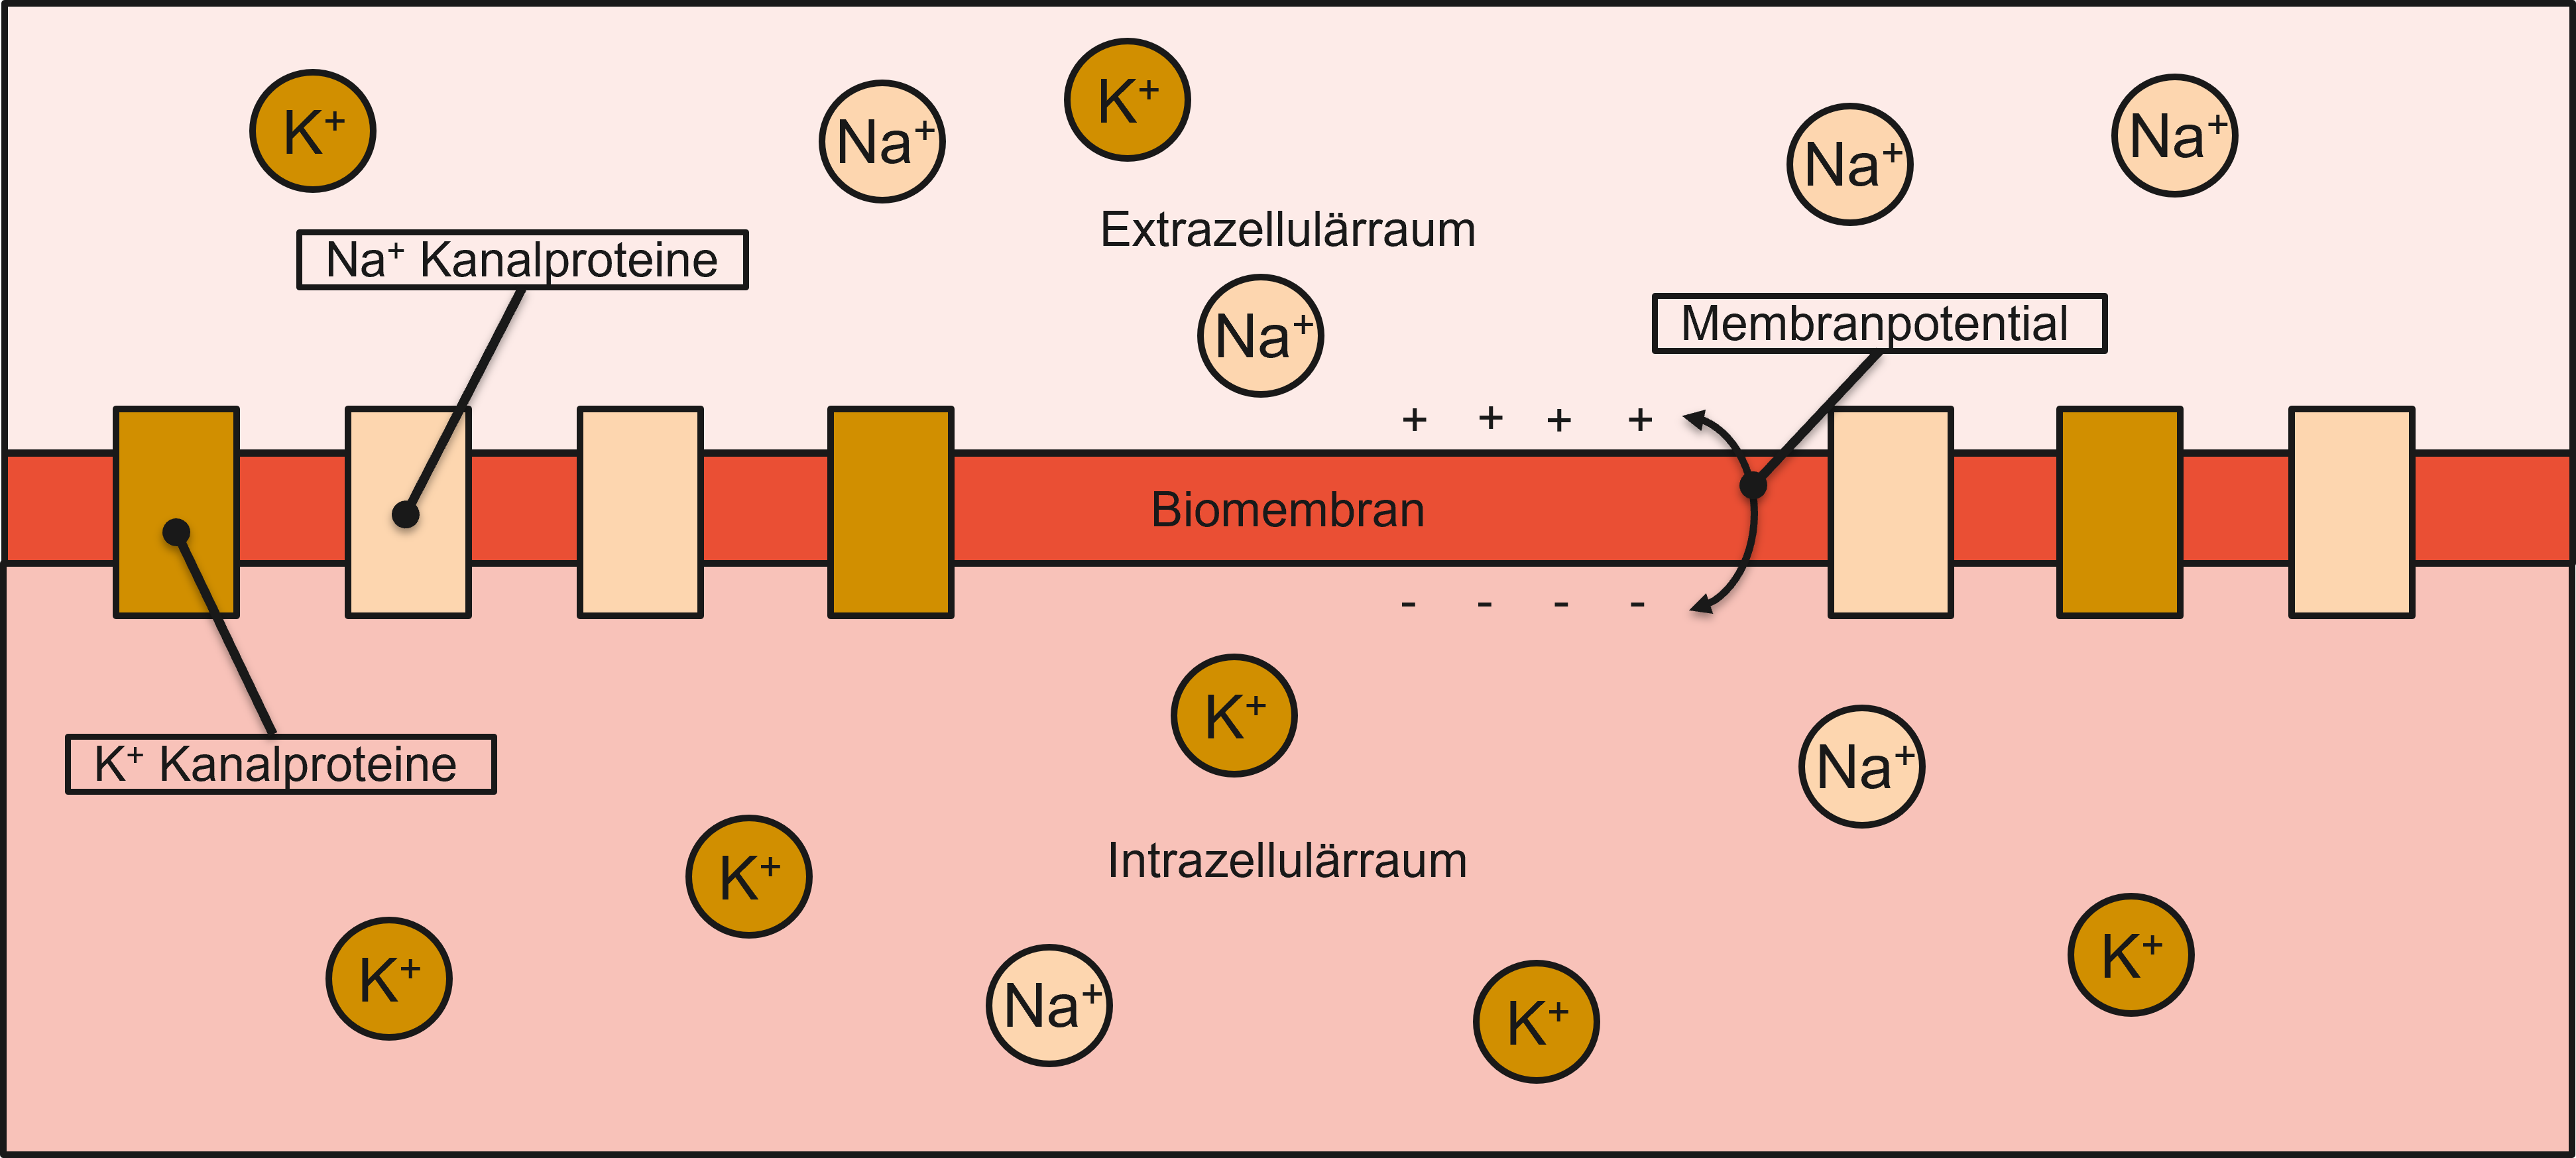
\includegraphics[width=0.9\textwidth]{papers/nerven/Bilder/Vorgang1.png}
    \caption{Ruhezustand}
    \label{fig:Ruhezustand}
\end{figure}
\noindent
Die Ladung von Zellinnerem und Zelläusserem wird durch die Verteilung von positiv geladenen Ionen gesteuert.
Die wichtigsten Ionen dafür sind Kalium- und Natriumionen. 
Durch eine sogenannte Ionenpumpe, wird ermöglicht, dass sich Ruhezustand der Zelle mehr Kaliumionen im Zellinneren und mehr
Natriumionen im Zelläusseren befinden.
Da Kaliumionen eine grössere Ladung als Natriumionen besitzen ergibt sich so das negatives Membranpotential von -70
Millivolt.
Die Zellwand besteht aus einer Biomembran, die für Moleküle und Ionen undurchlässig ist.
In der Zellwand befinden sich jedoch Kanalproteine, die bei der richtigen Anregung spezifische Ionen durch die
Biomembran transportieren können.
\noindent
Wenn die Nervenzelle, wie in Abbildung \ref{fig:Anregung} extern angeregt wird, öffnen sich einige Natriumkanalproteine und transportieren so Natriumionen in
die Nervenzelle.
Durch die Natriumionen vergrössert sich die Ladung der Nervenzelle und das Membranpotential wird somit grösser.
\begin{figure}[H]
    \centering
    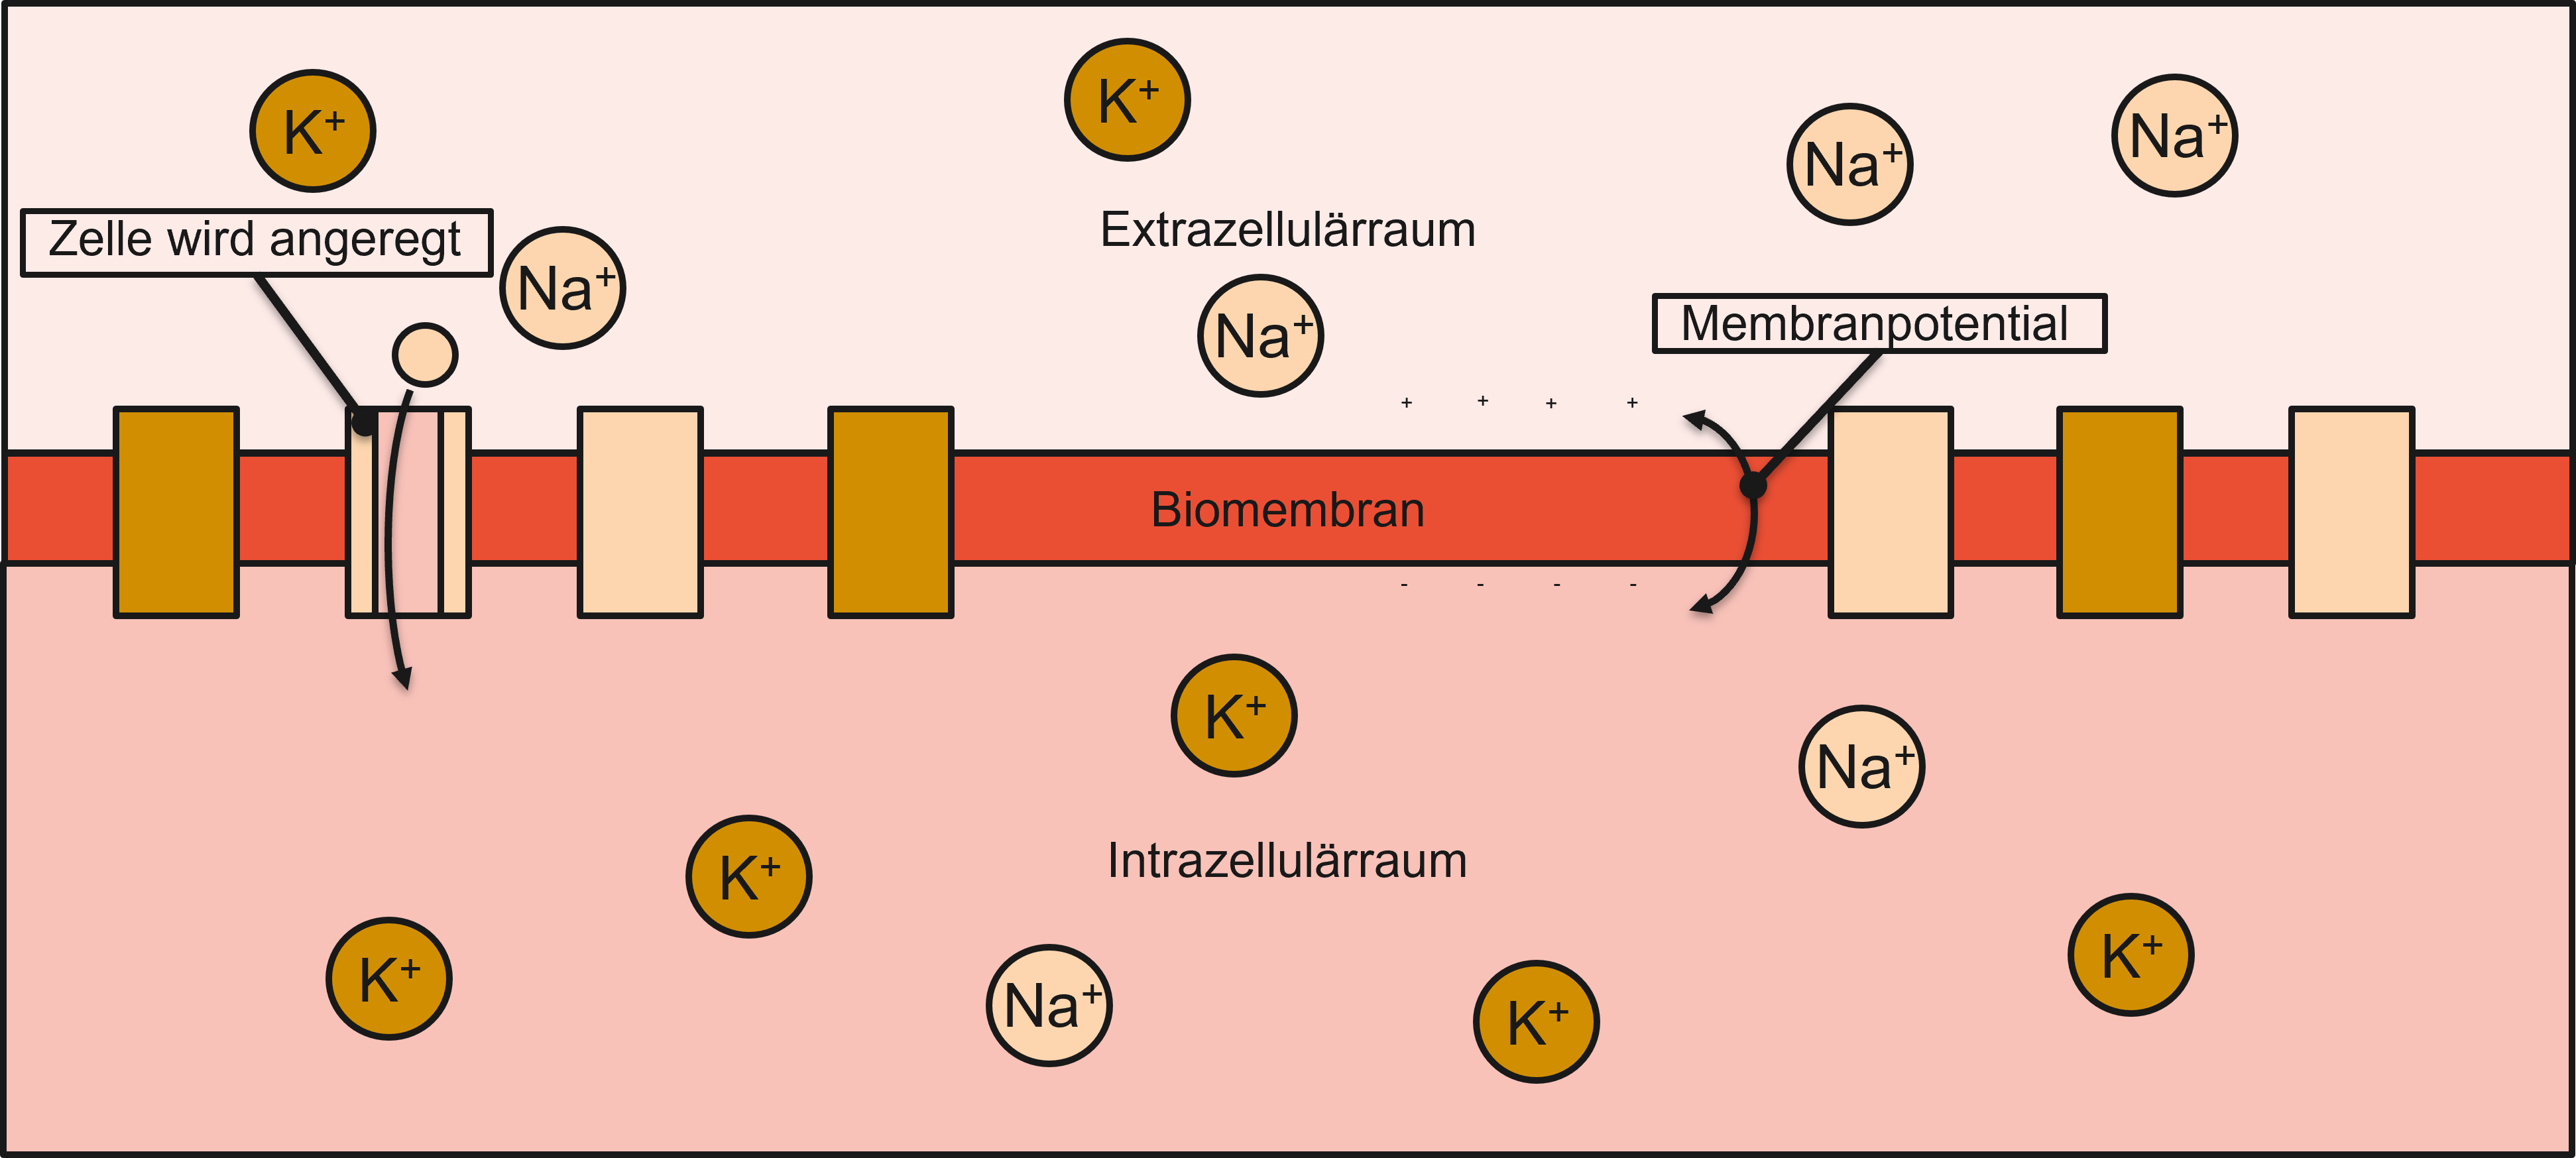
\includegraphics[width=0.9\textwidth]{papers/nerven/Bilder/Vorgang2.png}
    \caption{Anregung}
    \label{fig:Anregung}
\end{figure}
\noindent
Sobald das Membranpotential grösser als der Schwellenwert von -50 Millivolt ist, öffnen sich wie in Abbildung
\ref{fig:Depolarisation} erkennbar schlagartig viele
Natriumkanalproteine und transportieren noch mehr Natriumionen in die Nervenzelle.
Durch diese sogenannte Depolarisation erhöht sich die Ladung der Nervenzelle noch stärker und das Membranpotential erreicht ein Maximum. 
\begin{figure}[H]
    \centering
    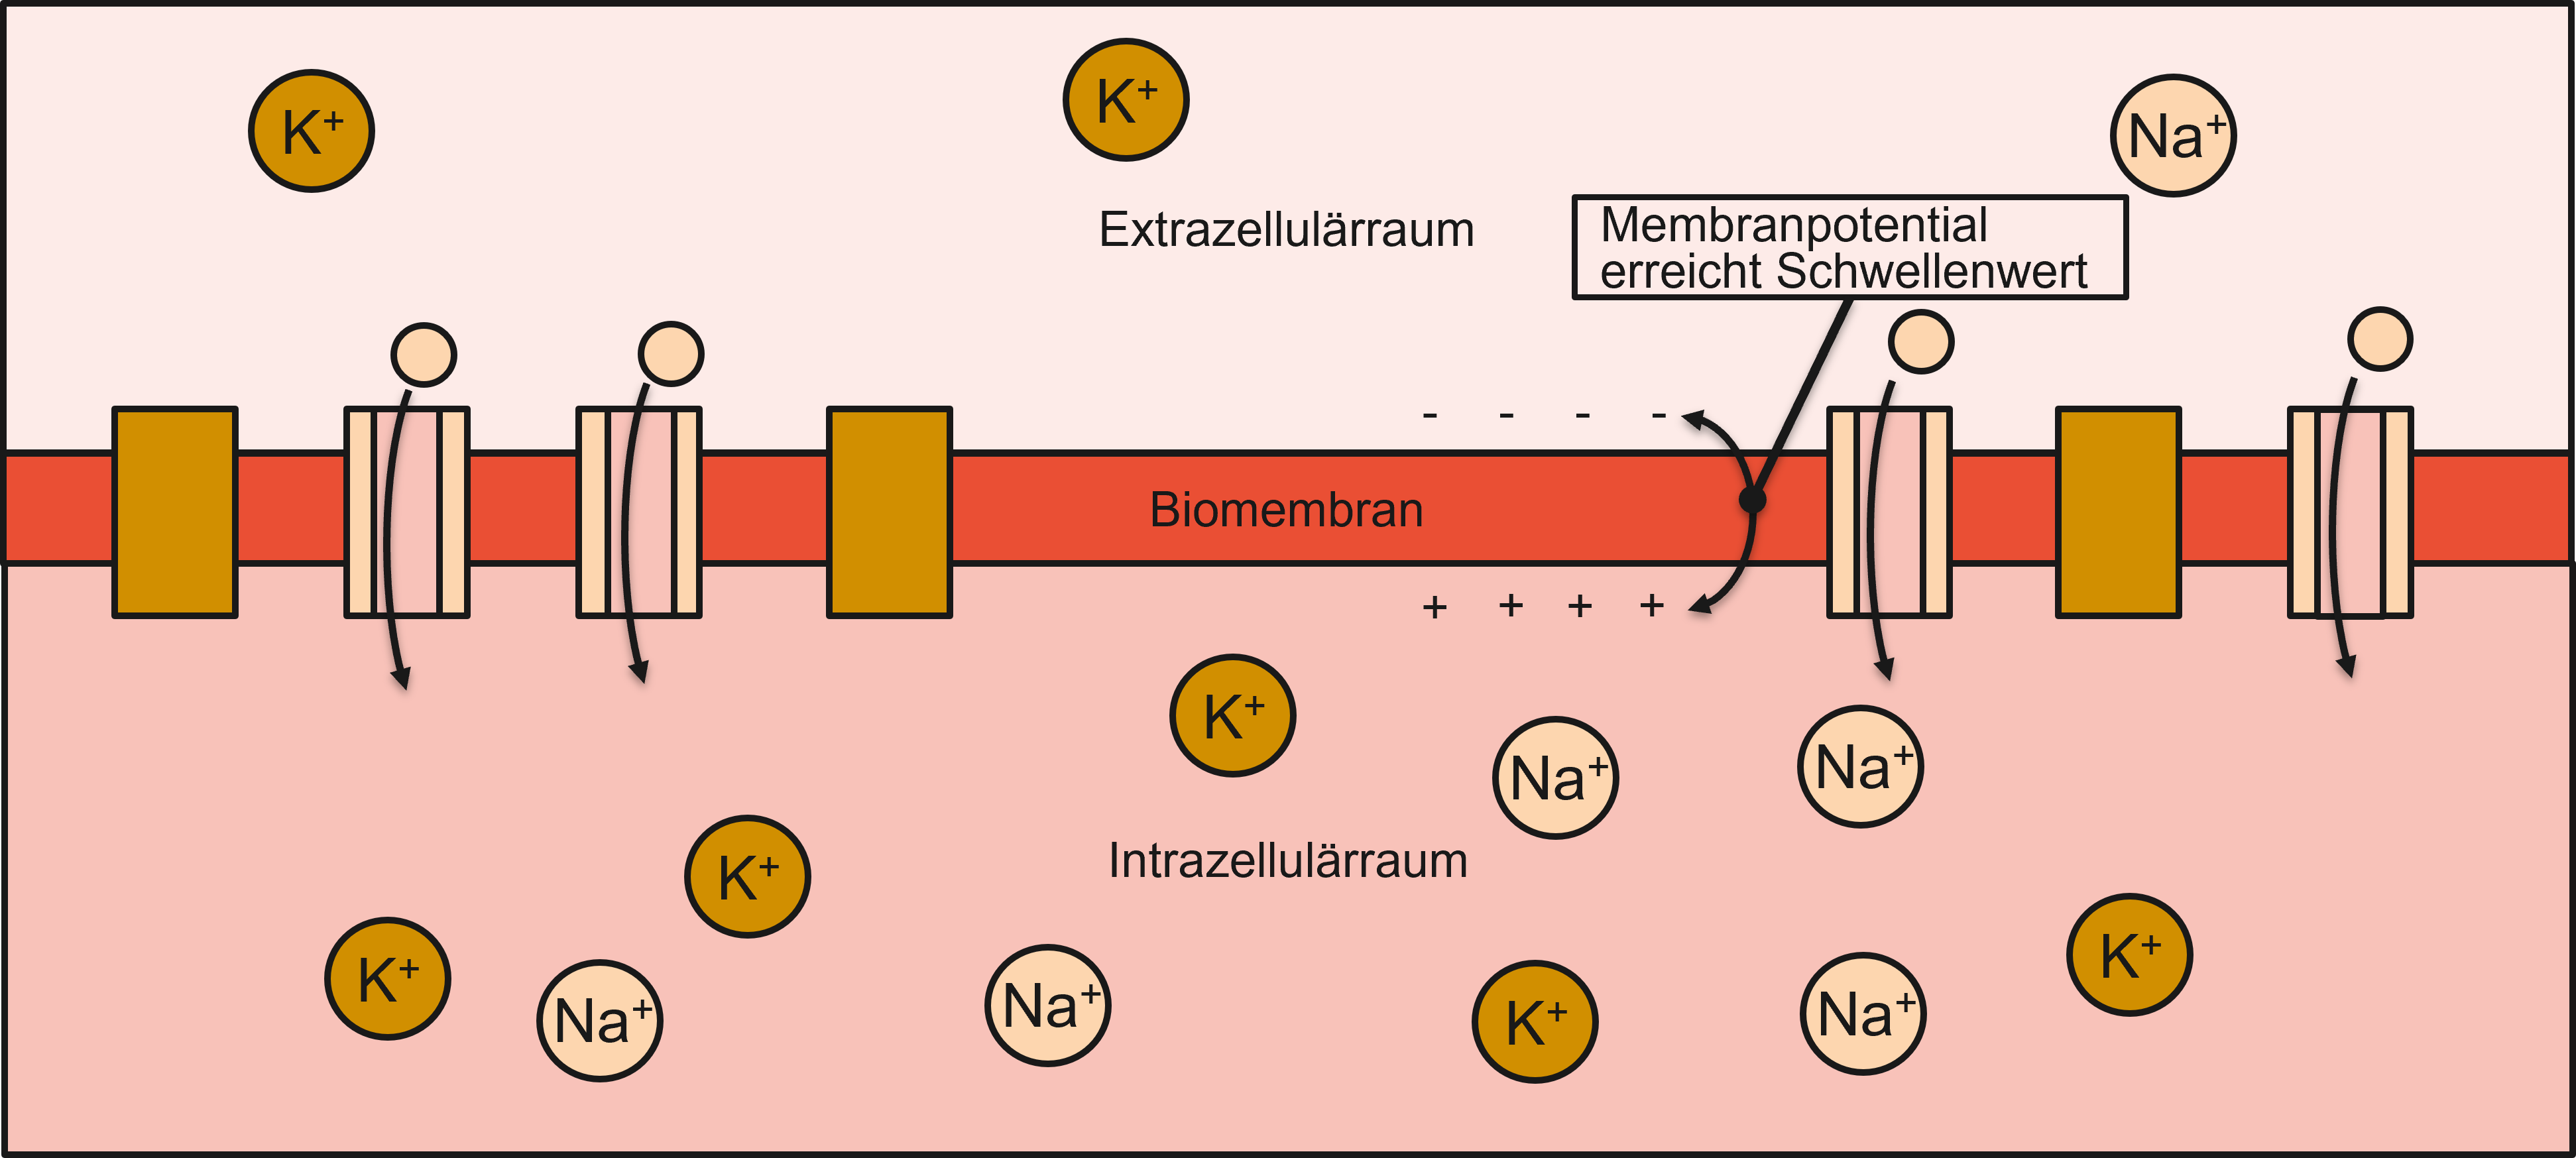
\includegraphics[width=0.9\textwidth]{papers/nerven/Bilder/Vorgang3.png}
    \caption{Depolarisation}
    \label{fig:Depolarisation}
\end{figure}
\noindent
Sobald das Membranpotential sein Maximum erreicht schliessen sich die Natriumkanalproteine und dafür öffnen sich die
Kaliumkanalproteine.
Wie in Abbildung \ref{fig:Repolarisation} ersichtlich strömen viele Kaliumionen aus der Nervenzelle hinaus.
In dieser Repolarisation nimmt deshalb das Membranpotential schlagartig wieder ab.
\begin{figure}[H]
    \centering
    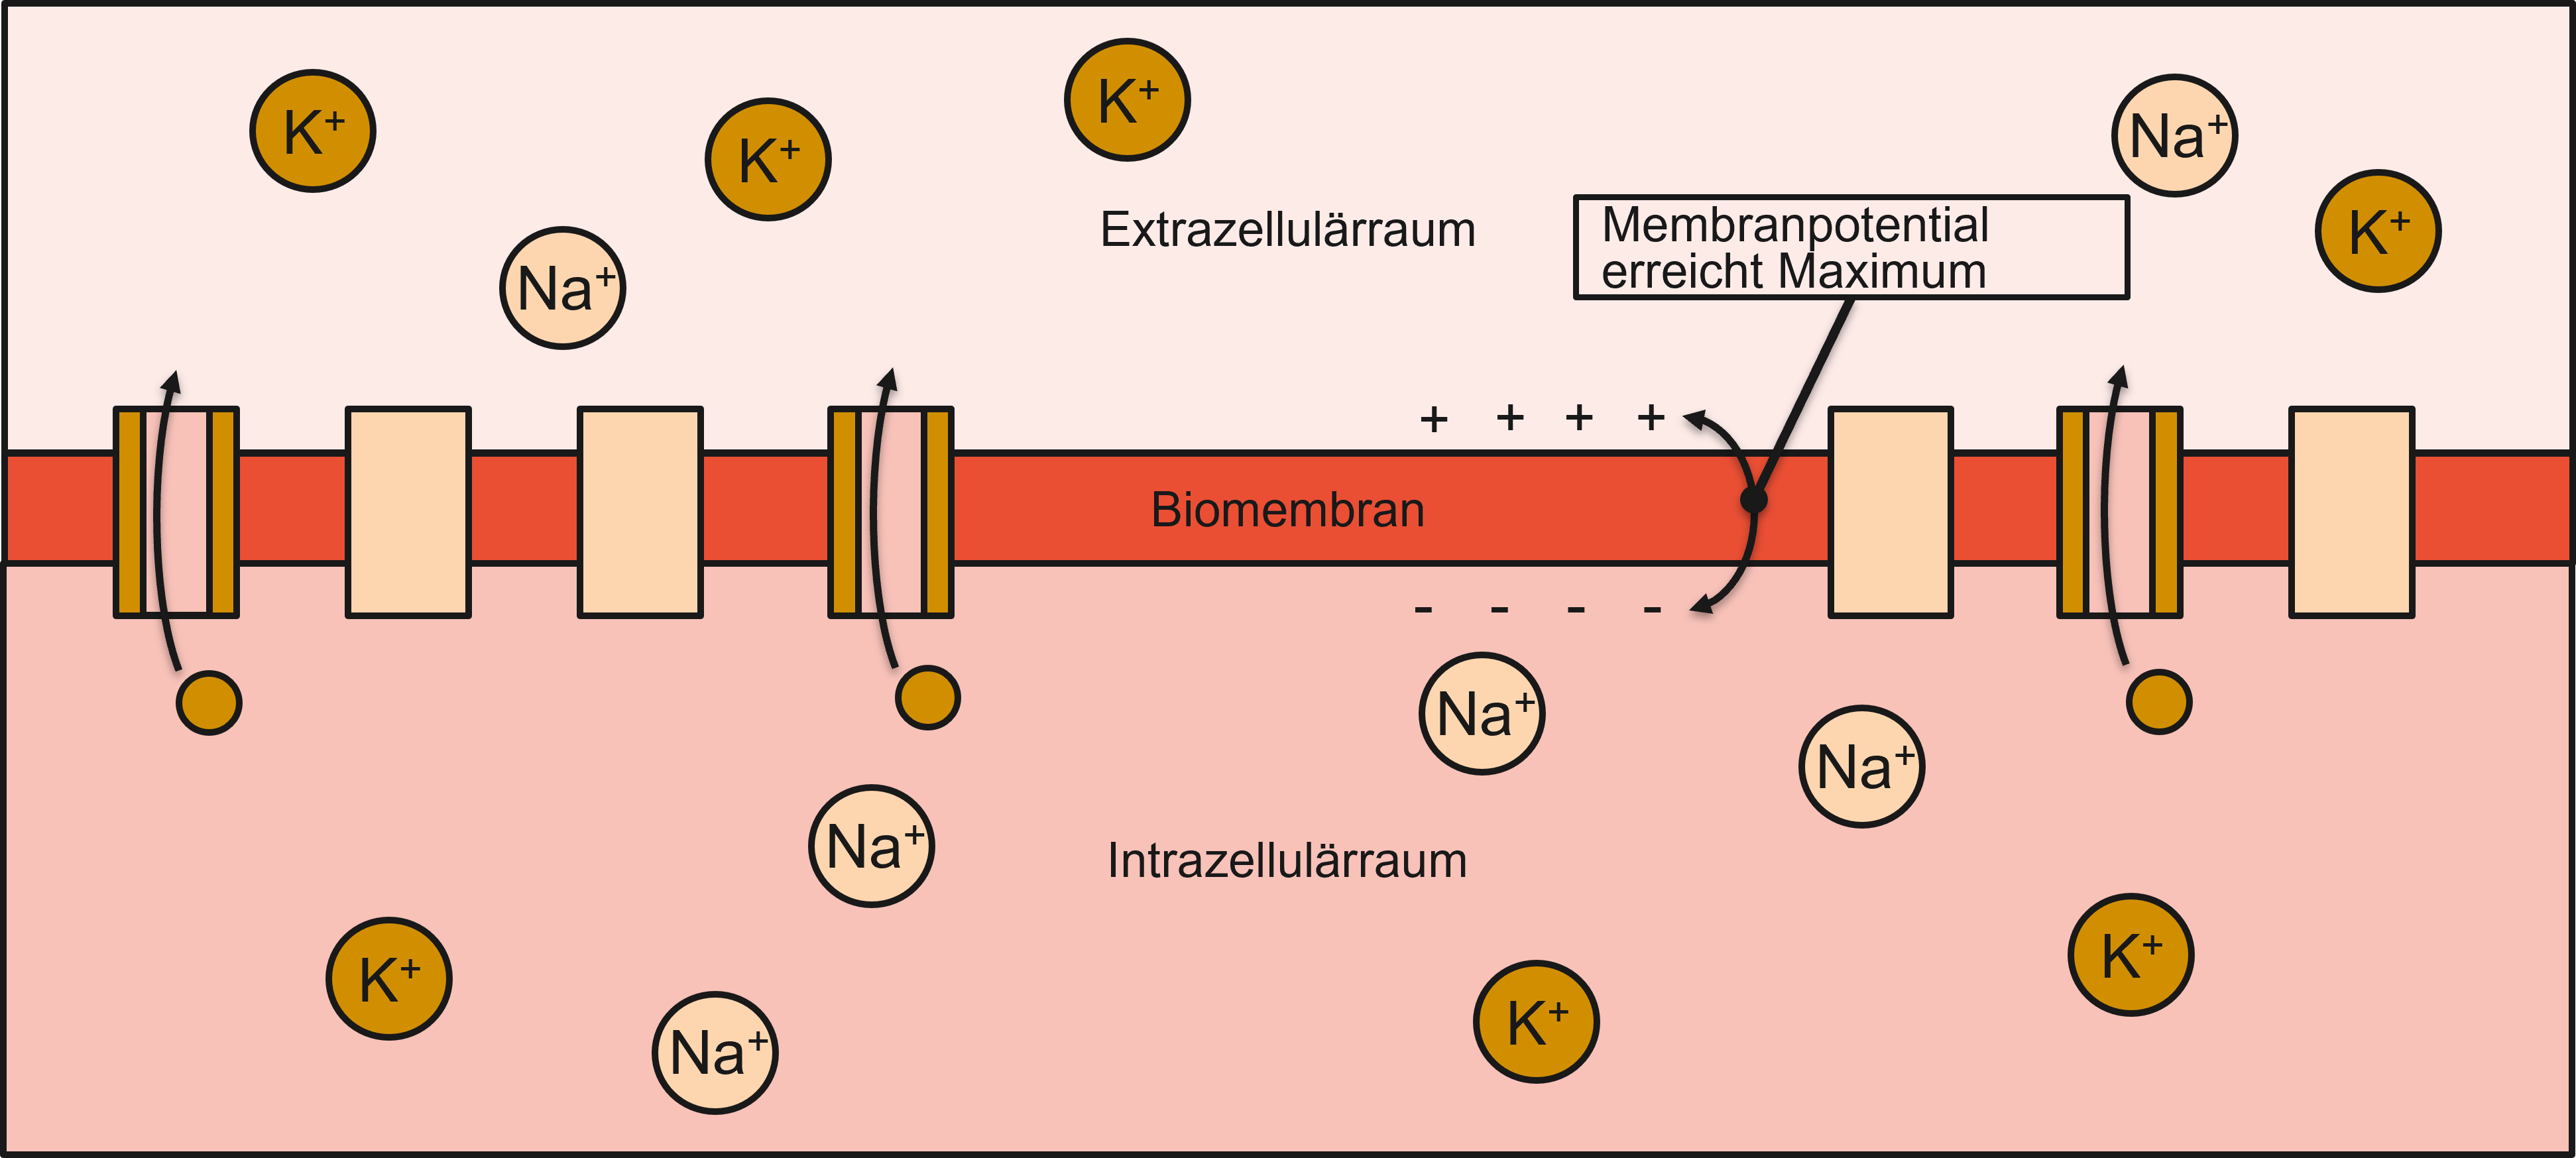
\includegraphics[width=0.9\textwidth]{papers/nerven/Bilder/Vorgang4.png}
    \caption{Repolarisation}
    \label{fig:Repolarisation}
\end{figure}
\noindent
Nachdem das Membranpotential wieder abgenommen hat, muss die Nervenzelle wieder in den Ruhezustand gelangen, dies nennt
man Hyperpolarisation.
Dafür öffnen sich, wie in Abbildung \ref{fig:Hyperpolarisation} ersichtlicht Kanalproteine für beide Ionen und durch die
Ionenpumpe strömen Kaliumionen in und Natriumionen aus der Zelle.
Durch die ungleiche Verteilung von Natrium- und Kaliumionen ensteht so wieder ein negatives Membranpotential an der Zellenwand.
\begin{figure}[H]
    \centering
    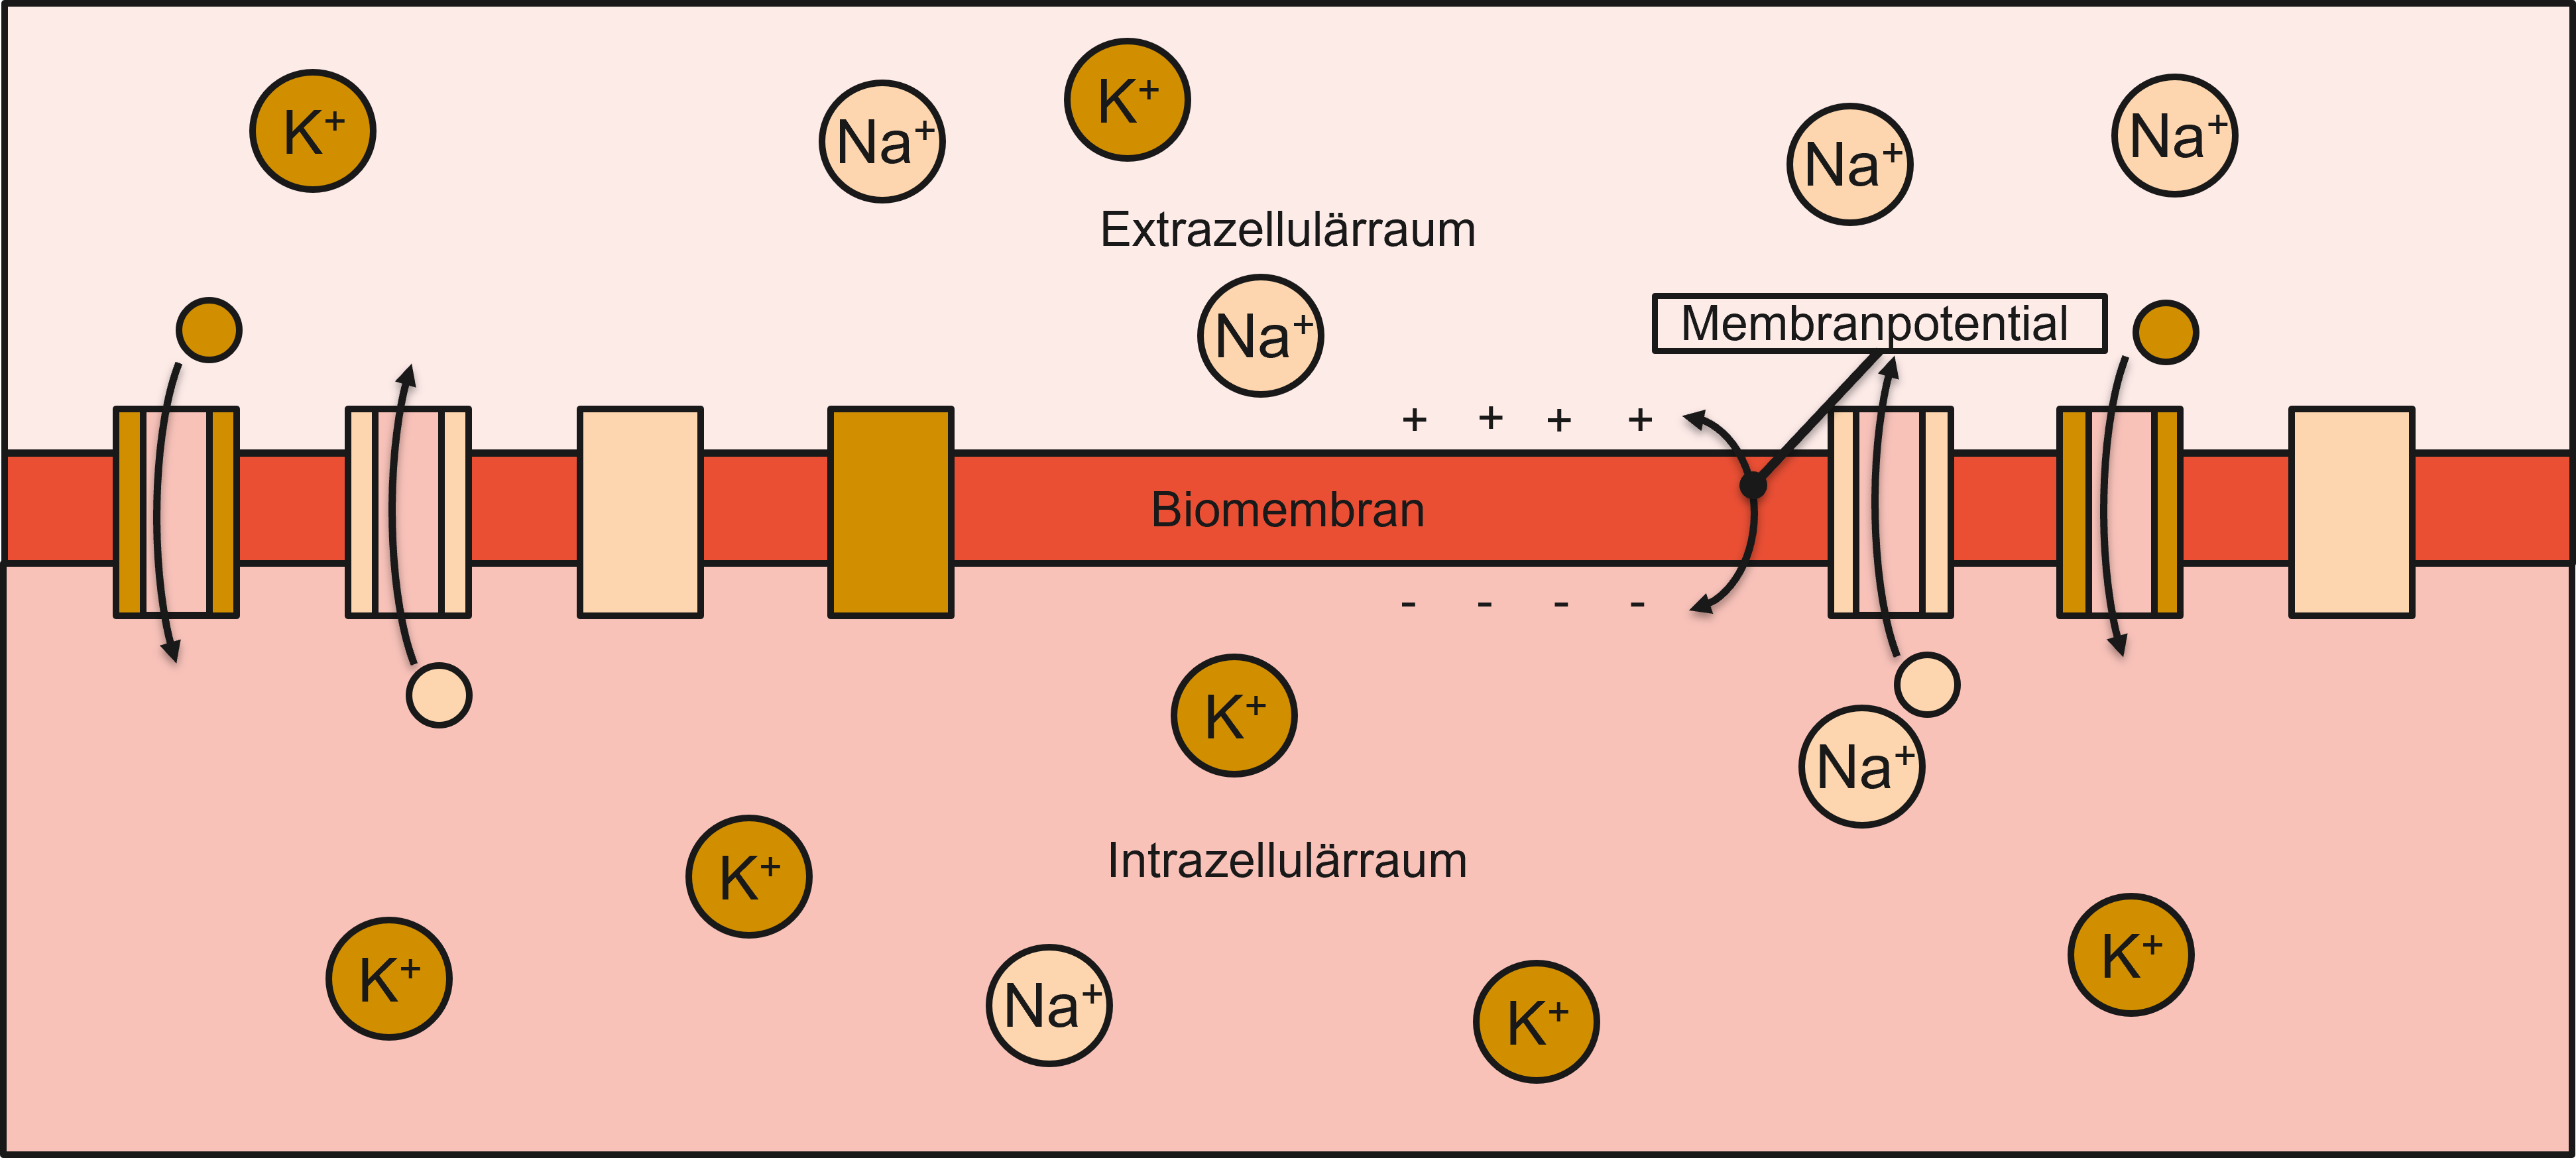
\includegraphics[width=0.9\textwidth]{papers/nerven/Bilder/Vorgang5.png}
    \caption{Hyperpolarisation}
    \label{fig:Hyperpolarisation}
\end{figure}

\section{Verhalten bei Anregung}
\subsection{Formelparameter}
In den vorigen Kapiteln wurde die Parameter der Nullklinien des Fitzhugh-Nagume Modells folgendermassen definiert.
\(a = -0.7, b = 0.8, \epsilon = 0.8, I = 0\), somit werden aus den allgemeinen Nullklinien, \( w = v - \frac{v^3}{3} + I\)
und \(w = \frac{v + a}{b}\) die spezifischen Nullklinien \( w = v - \frac{v^3}{3}\)
und \(w = \frac{v + 0.7}{0.8}\).
Der stationäre Punkt, welcher von Objekten im Vektorfeld angestrebt werden befindet sich bei \((1.2 |-0.6)\).
Der Parameter I ist als 0 definiert, dies bedeutet es findet keine Anregung statt.
In Abbildung \ref{fig:Parameter} sind das Vektrofeld und die Nullklinien erkennbar, wenn das Modell nicht angeregt wird.
\begin{figure}[H]
    \centering
    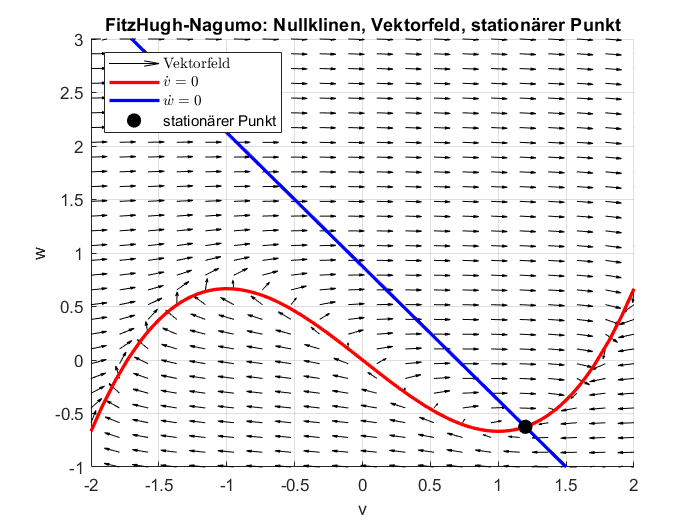
\includegraphics[width=0.9\textwidth]{papers/nerven/Bilder/Anregung1.png}
    \caption{Parameter}
    \label{fig:Parameter}
\end{figure}
\subsection{Schwache Anregung}
Wenn das Nullklinienmodell angeregt werden soll, muss der Parameter I verändert werden.
Beispielweise kann I = 0.1 Volt definiert werden.
Dadurch wird die v-Nullklinie um 0.1 in positive w-Richtung verschoben.
Somit verändern sich die Nullklinien zu \( w = v - \frac{v^3}{3} + 0.1\)
und \(w = \frac{v + 0.7}{0.8}\) und der stationäre Punkt wandert zu \((1.1 |-0.5)\).
Der ursprüngliche stationäre Punkt ist jetzt nicht mehr stabil und wird vom Vektorfeld in den neuen stationären Punkt
gezwungen.
Dies geschieht entlang des Vektorfelds, was bei dieser schwachen Anregung nur eine kurze Trajektorie ergibt.
In Abbildung \ref{fig:schwacheAnregung} lässt sich die Trajektorie zwischen den stationären Punkten erkennen, sowie
deren Auslenkung in v-Richtung.
Da die Anregung von I = 0.1 sehr schwach ist, fällt auch die Auslenkung der Trajektorie in v-Richtung mit 0.2 klein aus und
nimmt sofort wieder ab. 
Dieser Effekt tritt auf, wenn die Nervenzelle mit einer Spannung unterhalb der Schwellenspannung angeregt wird.
\begin{figure}[H]
    \centering
    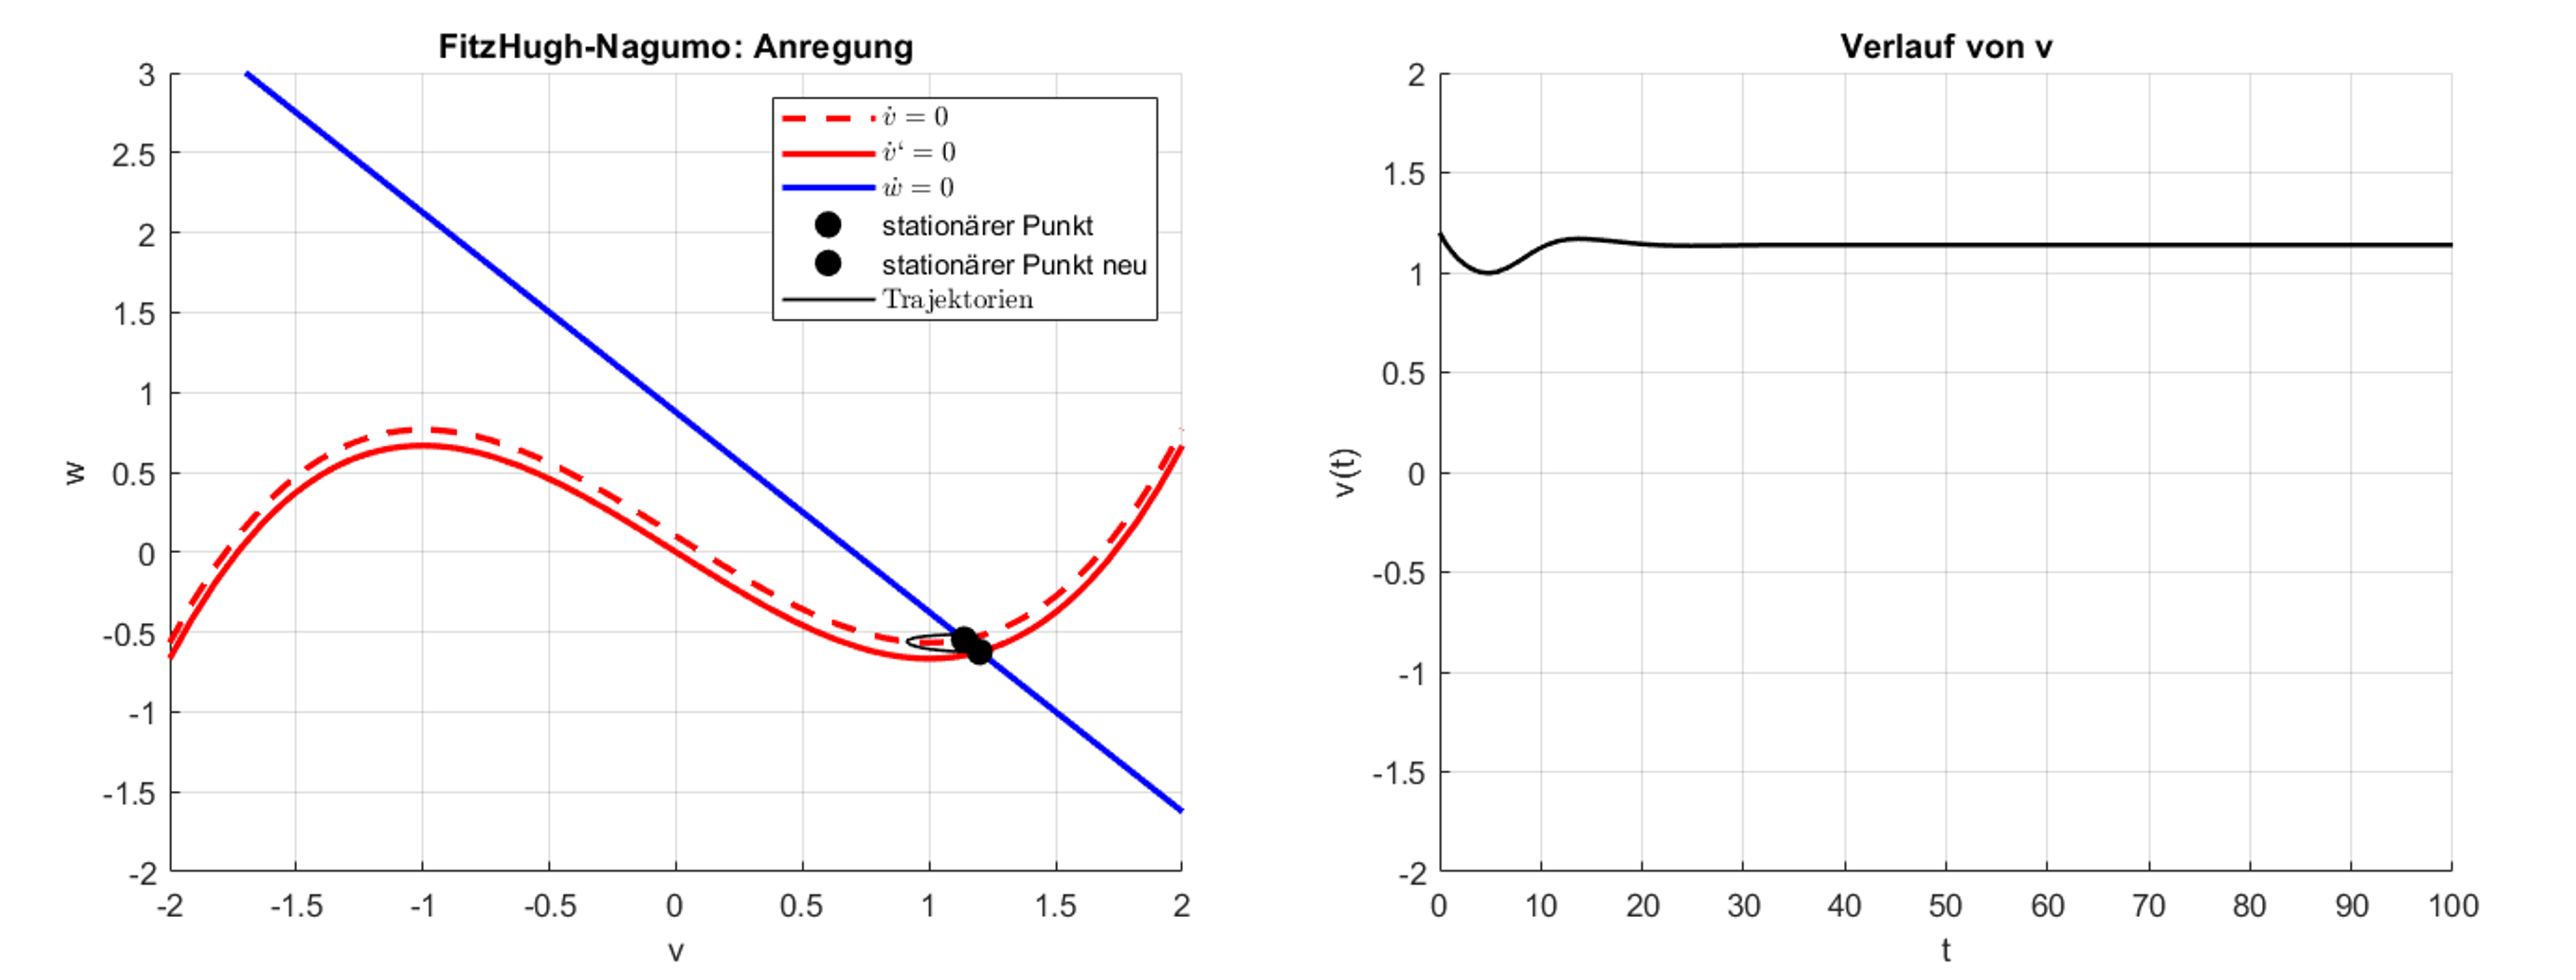
\includegraphics[width=0.9\textwidth]{papers/nerven/Bilder/schwacheAnregung.png}
    \caption{Schwache Anregung}
    \label{fig:schwacheAnregung}
\end{figure}
\subsection{Starke Anregung}
Um den Effekt, der bei einer Nervenzelle bei Anregung über der Schwellenspannung auftritt, beobachten zu können, muss
der Parameter I erhöht werden.
Beispielweise wird hier I = 0.3 Volt definiert.
Dadurch wird die v-Nullklinie um 0.3 in positive w-Richtung verschoben.
Somit verändern sich die Nullklinien zu \( w = v - \frac{v^3}{3} + 0.3\)
und \(w = \frac{v + 0.7}{0.8}\) und der stationäre Punkt wandert zu \((1 |-0.3)\).
Der ursprüngliche stationäre Punkt ist wird wieder instabil und vom Vektorfeld in den neuen stationären Punkt
gezwungen.
Dies geschieht entlang des Vektorfelds, was bei dieser stärkeren Anregung eine lange Trajektorie ergibt.
In Abbildung \ref{fig:starkeAnregung} lässt sich die Trajektorie zwischen den stationären Punkten erkennen, sowie
deren Auslenkung in v-Richtung.
Durch das Vektorfeld muss der ursprüngliche stationäre Punkt, bei einer Anregung von I = 0.3 eine grosse Kurve
beschreiben um den neuen stationären Punkt zu erreichen.
Die Auslenkung in v-Richtung ist dadurch mit -3 auch viel grösser und es lässt sich ein impulsartiger Verlauf erkennen.
\begin{figure}[H]
    \centering
    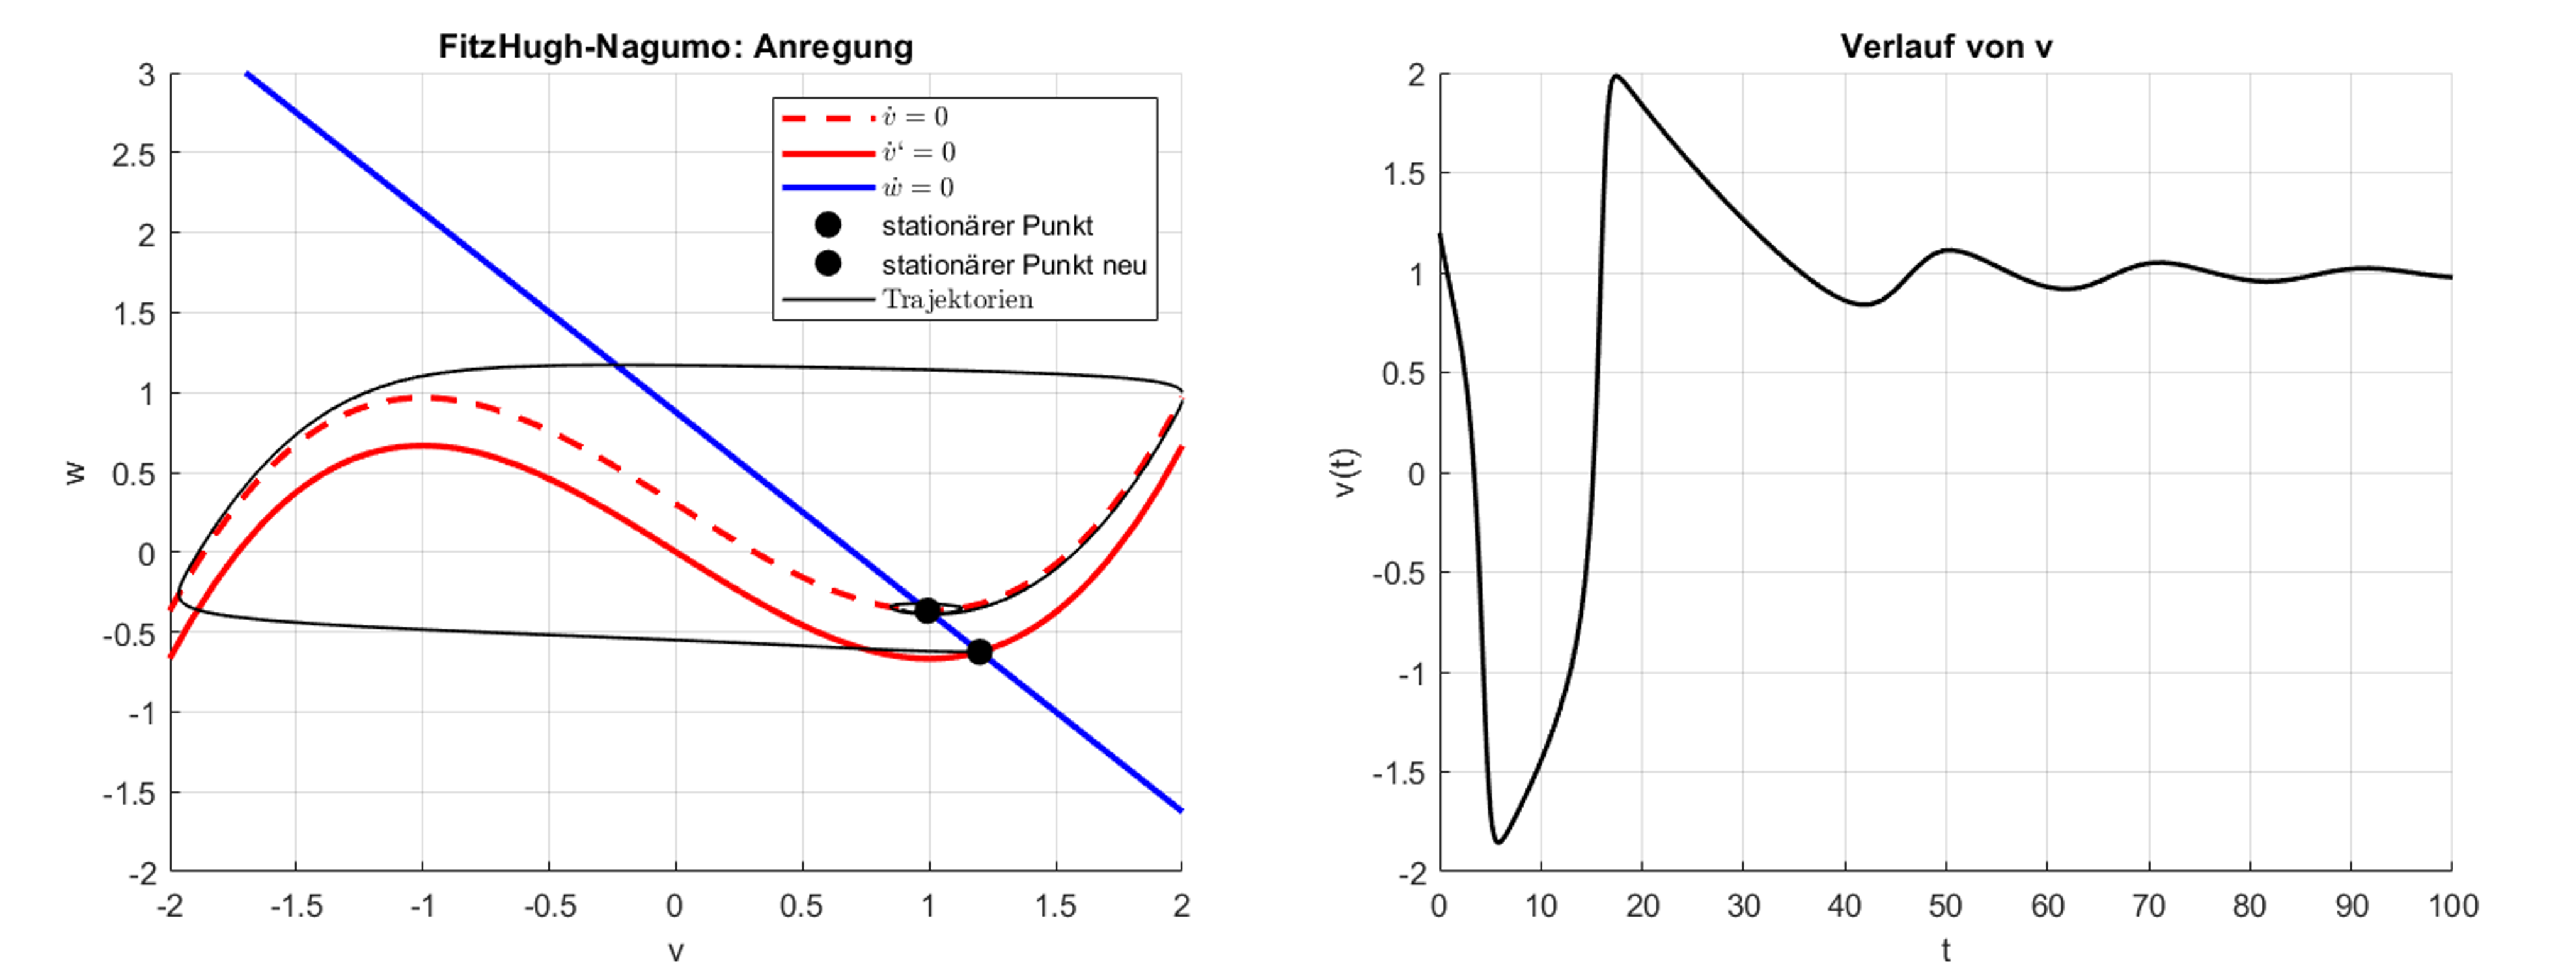
\includegraphics[width=0.9\textwidth]{papers/nerven/Bilder/starkeAnregung.png}
    \caption{Starke Anregung}
    \label{fig:starkeAnregung}
\end{figure}

\subsection{Vergleich mit Aktionspotential}
Den Verlauf der Auslenkung der Trajektorie in v-Richtung bei einer starken Anregung des Fitzhugh-Nagumo-Modells, lässt
sich mit dem Verlauf des Aktionspotentials der Nervenzelle vergleichen. 
In Abbildung \ref{fig:Vergleich} sind links die Auslenkung in v-Richtung und rechts der Verlauf des Aktionspotentials
erkennbar.
Der Verlauf der Auslenkung in v-Richtung ist an der v-Achse gespiegelt um die Abbildungen besser vergleichen zu können.
In der Abbildung lassen sich die einzelnen Phasen, Depolarisation, Repolarisation und Hyperpolarisation erkennen, die
sowohl im Verlauf der Auslenkung in v-Richtung und im Verlauf des Aktionspotentials auftreten.
Somit kann mit dem Nullklinienmodell des Fitzhugh-Nagumo-Modells der Verlauf des Aktionspotentials einer Nervenzelle
dargestelt werden.
\begin{figure}[H]
    \centering
    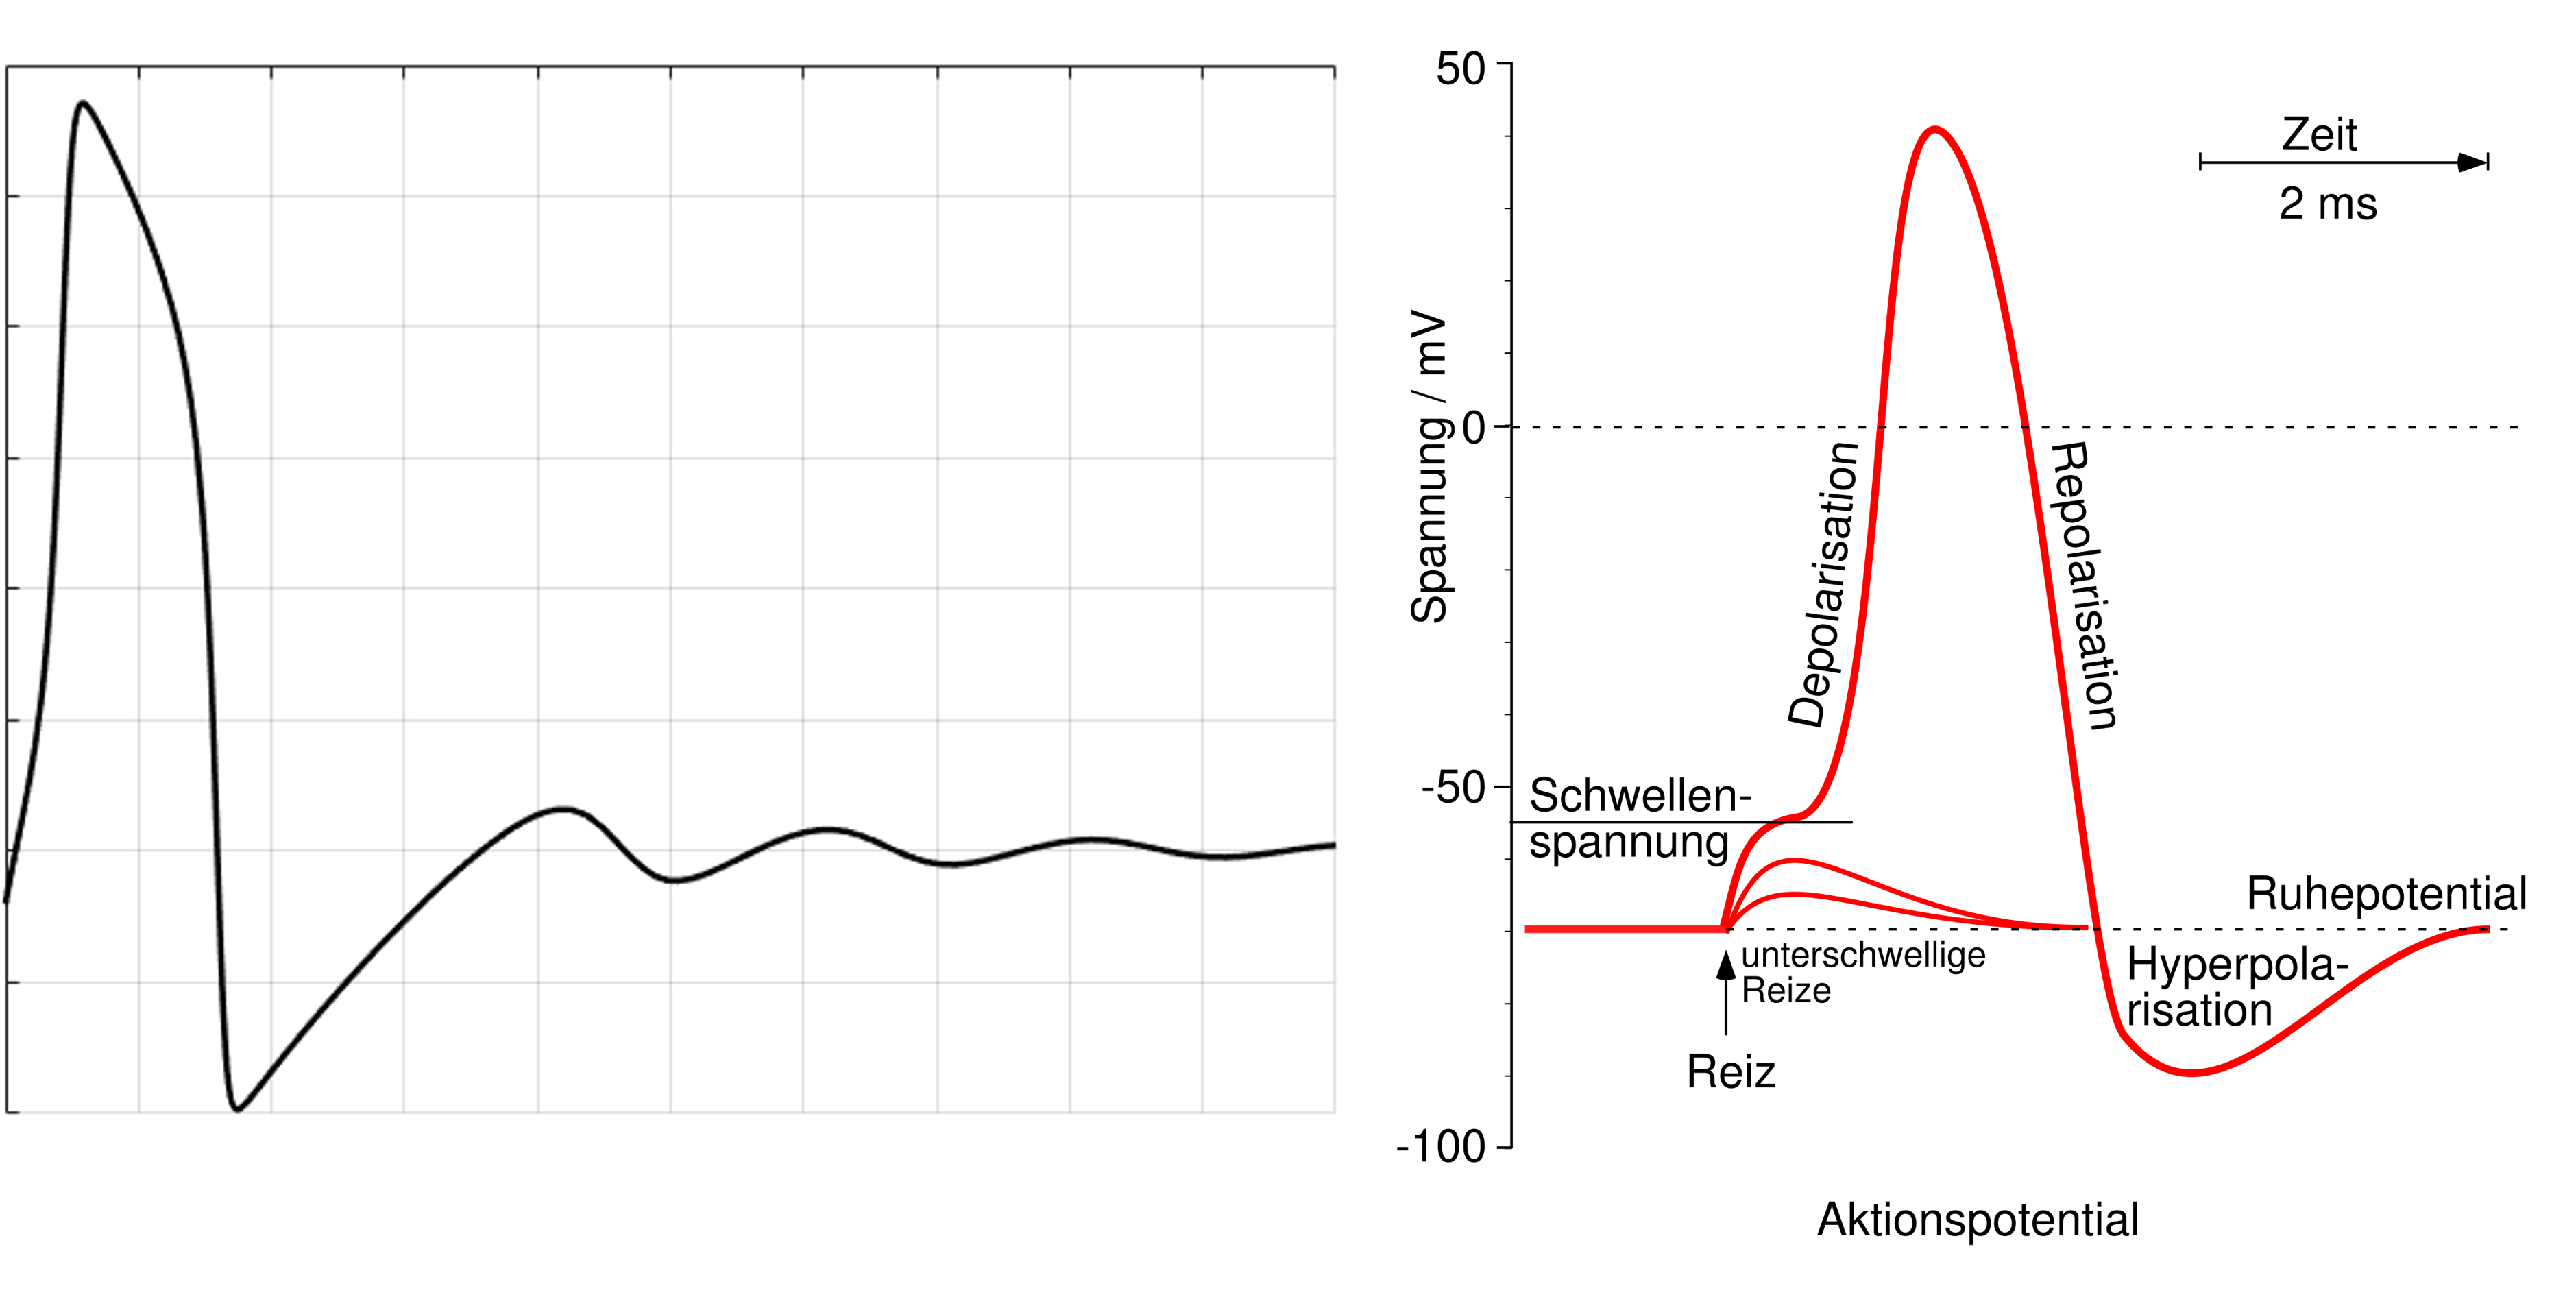
\includegraphics[width=0.9\textwidth]{papers/nerven/Bilder/Vergleich.png}
    \caption{Vergleich v-Auslenkung Aktionspotential}
    \label{fig:Vergleich}
\end{figure}
\section{Hodgkin-Huxley Modell}
\subsection{Einleitung}
Das Hodgkin-Huxley-Modell wurde 1952 von den britischen Physiologen Alan Hodgkin und Andrew Huxley entwickelt. Es beschreibt das elektrophysiologische Verhalten von Nervenzellen, genauer gesagt den Aktionspotentialverlauf entlang einer Nervenfaser. Das Modell basiert auf experimentellen Messungen am Riesenaxon des Tintenfisches und erklärt, wie sich die elektrische Spannung entlang einer Nervenzelle über die Zeit verändert. Dieses Modell wurde zum ersten Mal erfolgreich verwendet, um den komplexen Ionenfluss durch die Zellmembran quantitativ zu beschreiben. Es bildet die Grundlage für viele spätere Modelle wie das FitzHugh-Nagumo-Modell, welches in dieser Arbeit vertieft behandelt wird.
\subsection{Nutzen}
Der grösste Beitrag des Hodgkin-Huxley-Modells liegt in der mathematischen Beschreibung der biologischen Realität: Es verbindet biologische Prozesse wie Natrium- und Kaliumkanalbewegungen mit einem System nichtlinearer Differentialgleichungen. Das Modell erklärt das Zustandekommen eines Aktionspotentials und erlaubt Simulationen und Vorhersagen für Nervenreaktionen auf Reize. Es ist bis heute in der Neuroinformatik, Biophysik und mathematischen Neurowissenschaft von zentraler Bedeutung und diente als Grundlage für realistische neuronale Netzwerke.
\subsection{Mathematische Grundlagen}
Das Hodgkin-Huxley-Modell basiert auf der elektrischen Leitfähigkeit der Membrane und stellt die Nervenmembrane als ein elektrisches Schaltbild dar: bestehend aus einer Kapazität C_m, und mehreren stromleitenden Kanälen für spezifische Ionen.
Die fundamentale Gleichung ist der einzige Ausschnitt vom Hodgkin-Huxley-Modell welches aus natürlichen und biologischen Beobachtungen entstanden ist, die restlichen Gleichungen und Beobachtungen hängen nicht deutlich von molekularen Mechanismen zusammen.
\[
C_m \frac{dV}{dt} = I_{\text{ext}} - (I_{\text{Na}} + I_{\text{K}} + I_L)
\]

Dabei ist:

\begin{itemize}
	\item $V(t)$: Membranpotential (mV)
	\item $C_m$: Membrankapazität pro Fläche ($\mu$F/cm$^2$)
	\item $I_{\text{ext}}$: externer Reizstrom
	\item $I_{\text{Na}}, I_{\text{K}}$: Natrium- und Kaliumströme
	\item $I_L$: Leckstrom
\end{itemize}
\subsubsection{Ionenströme}
Die Ionenströme sind spannungs- und zeitabhängig. Sie folgen jeweils einer eigenen Formel:
\[
\begin{aligned}
	I_{\text{Na}} &= \bar{g}_{\text{Na}} \cdot m^3 h \cdot (V - E_{\text{Na}}) \\
	I_{\text{K}} &= \bar{g}_{\text{K}} \cdot n^4 \cdot (V - E_{\text{K}}) \\
	I_L &= \bar{g}_L \cdot (V - E_L)
\end{aligned}
\]

Erklärung:

\begin{itemize}
	\item $\bar{g}_{\text{Na}}, \bar{g}_{\text{K}}, \bar{g}_L$: maximale Leitfähigkeiten (Konstanten)
	\item $E_{\text{Na}}, E_{\text{K}}, E_L$: Umkehrpotentiale der Ionen
	\item $m, h, n$: \textbf{Torvariablen}, die zwischen 0 und 1 schwanken und die Öffnungswahrscheinlichkeit von Ionenkanälen angeben
\end{itemize}
Die Torvariablen m,h und n sind Variablen die keine reine biologische Überlegungen haben, sondern durch herumprobieren entstanden sind. Diese Torvariablen werden so angepasst das die Dynamik bei den Natrium- und Kaliumionenkanälen erklärt wird.
\subsubsection{Dynamik der Torvariablen}
Die Torvariablen folgen jeweils differentiellen Gleichungen 1. Ordnung, z. B.:
\[
\frac{dm}{dt} = \alpha_m(V) \cdot (1 - m) - \beta_m(V) \cdot m
\]

\begin{align}
	\frac{dn}{dt} &= \alpha_n (1 - n) - \beta_n n \tag{3.11} \\
	\frac{dm}{dt} &= \alpha_m (1 - m) - \beta_m m \tag{3.12} \\
	\frac{dh}{dt} &= \alpha_h (1 - h) - \beta_h h \tag{3.13}
\end{align}

Ähnliche Gleichungen gelten für dn dt und dh dt. Dabei sind αm alpha_mαm und βm beta_mβm spannungsgesteuerte Übergangsraten, die empirisch durch Hodgkin und Huxley bestimmt wurden.

Diese Differentialgleichungen beschreiben wie m,h und n jeweils vom Membranpotential V abhängig sind.
\subsubsection{Mathematische Einordnung der Gleichung}
Mathematisch handelt es sich beim Hodgkin-Huxley-Modell um ein System von vier gekoppelten nichtlinearen Differentialgleichungen:
•	Eine Gleichung für das Membranpotential V(t)
•	Drei Gleichungen für die Torvariablen m(t),h(t),n(t)
Es gehört zur Klasse der nichtlinearen dynamischen Systeme, genauer gesagt zu einem System von gewöhnlichen Differentialgleichungen. Die Nichtlinearität entsteht durch die Potenzen (z.B. m^3) und das Produkt der Torvariablen mit V.
\subsubsection{Fazit}
Das Hodgkin-Huxley-Modell ist nicht nur ein Meilenstein der Biologie, sondern auch ein Paradebeispiel dafür, wie mathematische Modellierung biologische Prozesse quantitativ erfassen kann. Die Gleichungen geben Verständnis über die Entstehung und Ausbreitung elektrischer Signale in Nervenzellen und sind bis heute unverzichtbar in der Neurophysik und mathematischen Biologie.
\section{FitzHugh-Nagumo-Modell}
Das FitzHugh-Nagumo-Modell ist eine mathematische Vereinfachung des Hodgkin-Huxley-Modells. Entwickelt wurde es in den 1960er-Jahren von Richard FitzHugh und Jinichi Nagumo, um die komplexe Dynamik des neuronalen Aktionspotentials auf ein qualitativ ähnliches, aber mathematisch reduziertes System zurückzuführen.
Das Modell abstrahiert die Nervenaktivität auf zwei Hauptvariablen:
1.	Das Membranpotential v(t)
2.	Eine Erholungsvariable w(t), die langsame Rückstellprozesse modelliert
Ziel war es, ein System zu formulieren, das zwar die fundamentalen Eigenschaften wie Reizantwort, Erregbarkeit und Rückkehr zum Ruhezustand bewahrt, aber deutlich einfacher zu analysieren ist. 
\subsubsection{Nutzen des FitzHugh-Nagumo-Modells}
Das FitzHugh-Nagumo-Modell erlaubt eine qualitative Analyse neuronaler Aktivität mit einfachen Mitteln:
•	Simulation von Aktionspotentialen
•	Beschreibung von Refraktärzeiten
•	Untersuchung der Stabilität von Ruhezuständen
•	Analyse von Schwellwertverhalten bei Reizen
•	Einsatz in räumlich ausgedehnten Modellen (z.B. als Reaktions-Diffusions-System für Ausbreitung von Signalen im Gewebe)
Gerade in der Mathematik ist das Modell besonders beliebt, da es sich ideal für phasenraumanalytische Methoden eignet – insbesondere für die Betrachtung von Nullklinen, Fixpunkten und Limitzyklen.
\subsubsection{Mathematische Beschreibung des Modells}
Das FitzHugh-Nagumo-Modell besteht aus einem System zweier gekoppelter nichtlinearer Differentialgleichungen 1. Ordnung:
Diese Differentialgleichung wurden aus der fundamtalen Formel vom Hodkin-Huxley-Modell hergeleitet, jedoch ist diese sehr komplex und wird in der Arbeit nicht weiter erklärt. Aus der fundamentalen Formel vom Hodkin-Huxley-Modell wurden diese zwei gekoppelten nichtlinearen Differentialgleichung 1.Ordnung:
\[
\begin{aligned}
	\frac{dv}{dt} &= v - \frac{v^3}{3} - w + I_{\text{ext}} \\
	\frac{dw}{dt} &= \varepsilon (v + a - b w)
\end{aligned}
\]

\textbf{Bedeutung der Variablen:}

\begin{itemize}
	\item $v(t)$: Membranpotential (schnelle Variable)
	\item $w(t)$: Erholungsvariable (langsame Variable)
	\item $I_{\text{ext}}$: externer Reiz
	\item $\varepsilon \ll 1$: kleine Konstante, die die Zeitskalen trennt (Langsamkeit von $w$)
	\item $a, b$: Systemparameter, die die Dynamik und Stabilität beeinflussen
\end{itemize}
Das ist ein 2-Dimensionales-System, also ebenes System von gewöhnlichen Differentialgleichungen. Dies veringert den mathematischen Aufwand und macht es uns sehr einfach Eigenschaften mithilfe des Modells zu indentifizieren.
Mit w und v als stetig und differenzierbar sind die Ergebnisse mithilfe von Nullklinien sehr leicht indentifizierbar.
Interpretation:
•	Die erste Gleichung beschreibt die schnelle Aktivierung des Neurons: sie enthält eine nichtlineare Rückkopplung durch den Term v^3, die für die typische „Spike“-Form des Aktionspotentials sorgt.
•	Die zweite Gleichung reguliert die langsame Erholung und Rückführung zum Ruhezustand.
\subsubsection{Mathematische Einordnung}
Das FitzHugh-Nagumo-Modell ist ein typisches Beispiel für ein Relaxationsoszillator-System, bei dem zwei Variablen auf unterschiedlichen Zeitskalen miteinander gekoppelt sind. Solche Systeme sind bekannt für:
•	Sprunghaftes Verhalten (z.B. plötzlicher Aktionspotentialanstieg)
•	Rückkehr zum Ausgangszustand (Refraktärphase)
•	Nichtlineare Dynamik mit Sättigung und Schwellenwertverhalten
Mathematisch ist es ein nichtlineares ODE-System (System gewöhnlicher Differentialgleichungen) und wird häufig mit Phasenporträts analysiert.
\subsubsection{Analyse der Nullklinen}
Die Nullklinen sind die geometrischen Orte im Phasenraum (v,w), an denen sich die jeweiligen Zeitableitungen nicht verändern (also gleich null sind). Sie sind ein zentrales Werkzeug zur Analyse des Systems.
\textbf{v-Nullkline:} $\dfrac{dv}{dt} = 0$

Setze:
\[
v - \frac{v^3}{3} - w + I_{\text{ext}} = 0
\]

Nach $w$ umgestellt:
\[
w = v - \frac{v^3}{3} + I_{\text{ext}}
\]

Das ist eine \textbf{kubische Kurve} im Phasenraum, typischerweise mit \textbf{S-Form}.  
Sie gibt an, wo das Membranpotential im Gleichgewicht ist (für festes $w$).

\vspace{1em}

\textbf{w-Nullkline:} $\dfrac{dw}{dt} = 0$

Setze:
\[
\varepsilon (v + a - b w) = 0 \Rightarrow v + a - b w = 0 \Rightarrow w = \frac{v + a}{b}
\]

Das ist eine \textbf{lineare Gerade} im Phasenraum.  
Sie gibt an, wo sich die Erholungsvariable im Gleichgewicht befindet (für festes $v$).
Der Schnittpunkt beider Nullklinen ist ein Gleichgewichtspunkt des Systems: Dort gilt sowohl dvdt=0\frac{dv}{dt} = 0dtdv=0 als auch dwdt=0\frac{dw}{dt} = 0dtdw=0. Dieser Punkt kann je nach Parametern stabil, instabil oder ein Oszillatorzentrum sein.
\subsubsection{Bedeutung}
Das Verhalten des Systems kann durch die Phasenporträtanalyse qualitativ vorhergesagt werden:
•	Wenn der Fixpunkt stabil ist, kehrt das System nach einem kleinen Reiz dorthin zurück → Ruhe.
•	Bei instabilem Fixpunkt (Sattel, Fokus) kommt es zu Limitzyklen → rhythmisches Feuern.
•	Der Verlauf der Trajektorien im Phasenraum zeigt den zeitlichen Verlauf des Aktionspotentials.
Die S-Form der v-Nullkline erzeugt Sprungdynamik:
•	Linker Ast: Ruhe
•	Mittlerer Ast: instabil (Schwellwert)
•	Rechter Ast: Aktivierung („Spike“)
Das FitzHugh-Nagumo-Modell ist eine elegante und reduktive Darstellung neuronaler Erregung, das die komplexe Biologie auf zwei mathematisch gut fassbare Prozesse reduziert. Seine Stärke liegt in der Analyse der Dynamik im Phasenraum, insbesondere über die Nullklinen und Fixpunkte. Es eignet sich hervorragend zur Simulation, Theoriebildung und Lehre – und bildet eine solide mathematische Brücke zwischen Biologie und dynamischer Systemtheorie.

%HAllo
%Ein paar Hinweise für die korrekte Formatierung des Textes
%
%%
% einleitung.tex -- Beispiel-File für die Einleitung
%
% (c) 2020 Prof Dr Andreas Müller, Hochschule Rapperswil
%
% !TEX root = ../../buch.tex
% !TEX encoding = UTF-8
%

\section{Grundlagen der Fourier-Analyse\label{fourier:section:teil0}}
\kopfrechts{Teil 0}

Die Fourier-Analyse ist ein sehr mächtiges Mittel in der Signal-Analyse. 
Einleitung...


% In der Wellenfunktion gibt es keine Sprünge -> Footnote alle Fourierreihen, welche wir brauchen konvergieren.

% Wo wollen wir damit hin? Ziel klar definieren. 
% Mögliche Strategie: Hinten beginnen.
% Da schreiben; klarer, was man vorher braucht und dann schrittweise aufführen. 
% Gedanken über Schritte machen.
% Bei Wellengleichung beginnen --> Fourierreihe --> 

\subsection{Fourierreihe\label{fourier:subsection:fourierreihe}}

Mit der Fourier-Reihe lassen sich periodisch wiederholende Funktionen, wie ein Rechteck- oder Dreiecksignal, mit skalierten Sinus- und Kosinus-Schwingungen darstellen.
Um die Reihe aufzustellen, braucht man nur 3 Koeffizienten zu bestimmen. 

\begin{itemize}
	\item $a_0$ ist der Mittelwert, der Funktion. 
	Dieser entspricht dem Integral über eine Periode und schliesslich geteilt durch die Periode. 
	
	\begin{equation}
		a_0 = \frac{1}{T} \int_{t_0}^{t_0 + T} f(t) \, dx
	\end{equation}
	
	\item $a_n$ beschreibt den geraden Anteil der Funktion.
	
	\begin{equation}
		a_n = \frac{2}{T} \int_{t_0}^{t_0 + T} f(t) \cos\left(\frac{2\pi n t}{T}\right) dt
	\end{equation}
	
	\item $b_n$ beschreibt den ungeraden Anteil der Funktion.
	
	\begin{equation}
		b_n = \frac{2}{T} \int_{t_0}^{t_0 + T} f(t) \sin\left(\frac{2\pi n t}{T}\right) dt
	\end{equation}
	
\end{itemize}

Mit allen Koeffizienten bestimmt lässt sich die ursprüngliche Funktion nachahmen.
Bei Funktionen mit Sprungstellen tritt das Gibbsche Phänomen auf.
Dies erklärt einen Überschwinger nach einem Sprung. Auch wenn man die unendliche Summe bildet, wird dieser Überschwinger nicht verschwinden.
Das $=$ Zeichen stimmt also nur bedingt.
Anhand der Abbildung ... sieht man sehr schön, wie die Rechteckfunktion mit Schwingungen nachgeahmt wird.

\[
f(t) = \frac{a_0}{2} + \sum_{n=1}^{\infty} \left( a_n \cos\left( \frac{2\pi n}{T} x \right) + b_n \sin\left( \frac{2\pi n}{T} x \right) \right)
\]

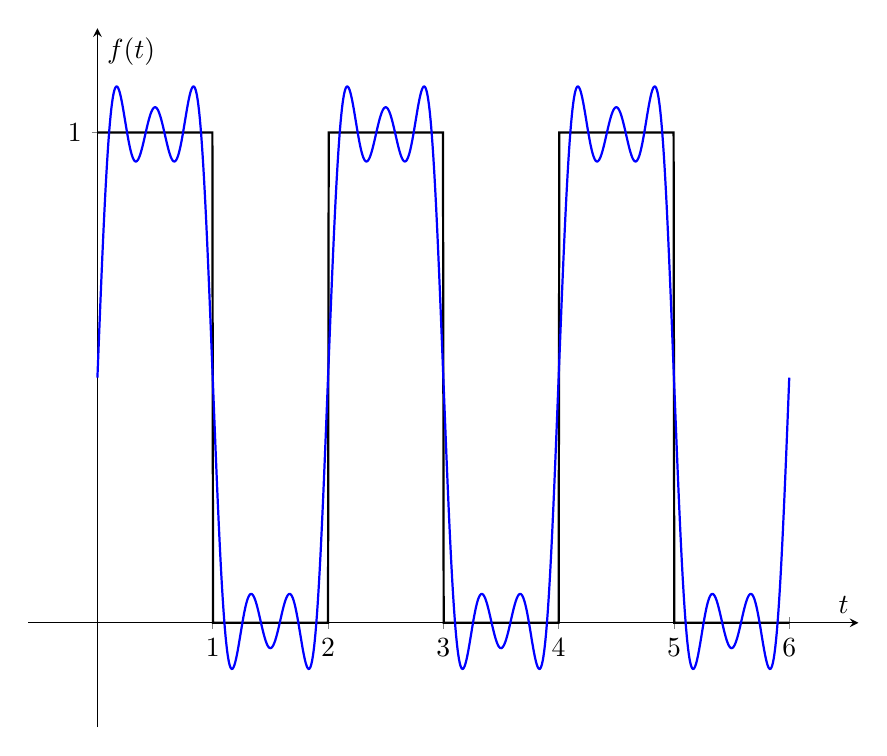
\begin{tikzpicture}
	\begin{axis}[
		axis lines = middle,
		xlabel = {$t$},
		ylabel = {$f(t)$},		
		domain=0:6,
		samples=1000,
		xtick={0,1,2,3,4,5,6},
		ytick={0,1},
		enlargelimits,
		width=\textwidth
		]
		\addplot[thick] {mod(floor(x),2) == 0 ? 1 : 0};
		\addplot[blue, thick] {(1/2) + 
			(2/pi)*sin(pi * deg(x)) + 
			(2/(3*pi))*sin(pi *3*deg(x)) +
			(2/(5*pi))*sin(pi *5*deg(x))};
	\end{axis}
\end{tikzpicture}

$a_0$ ist bei 


\subsection{Fouriertransformation\label{fourier:subsection:fouriertransformation}}


%%
% teil1.tex -- Beispiel-File für das Paper
%
% (c) 2020 Prof Dr Andreas Müller, Hochschule Rapperswil
%
% !TEX root = ../../buch.tex
% !TEX encoding = UTF-8
%
\section{Metrik und Hodge-Theorie 
\label{maxwell:section:teil1}}
\kopfrechts{Metrik und Hodge-Theorie}

\subsection{Minkowski Metrik}
In der speziellen Relativitätstheorie (SRT) wird die Minkowski-Metrik verwendet.
\index{spezielle Relativitätstheorie}%
\index{Relativitätstheorie, spezielle}%
\index{Minkowski-Metrik}%
Da es in der SRT keine Krümmung und Gravitation gibt, sind alle Elemente ausserhalb der Diagonale des metrischen Tensors null und somit ist die Raum-Zeit flach.
Zwei Signaturen sind üblich.
Einerseits gibt es die $({-}{+}{+}{+})$-Signatur, bei welcher die Zeitkomponente negativ und die Raumkomponenten positiv gezählt werden.
Andererseits gibt es die $({+}{-}{-}{-})$-Signatur, bei welcher die Zeitkomponente positiv und die Raumkomponenten negativ gezählt werden.
Beide Signaturen sind gleichwertig, solange man sich auf eine Metrik festlegt und diese konsequent beibehält.
Im Folgenden werden wir uns an die $({-}{+}{+}{+})$-Signatur halten.
Daher definieren wir den metrischen Tensor als
\begin{equation}
	g^{ik} = \begin{pmatrix}
		-1 & 0 & 0 & 0 \\ 0 & 1 & 0 & 0 \\ 0 & 0 & 1 & 0 \\ 0 & 0 & 0 & 1 
	\end{pmatrix}.
	\label{maxwell:section:teil1:metrik}
\end{equation}
Der Ausdruck für ein Linienelement in dieser Metrik ist definiert als
\begin{equation*}
	dl^2 = -(dx^0)^2 +(dx^1)^2+(dx^2)^2+(dx^3)^2.
\end{equation*}
Damit wir Raum und Zeit in dieser Metrik gleichartig behandeln können, wählen wir beim Übergang in physikalische Einheiten 
\begin{equation}
	\label{maxwell:koordinaten}
	x^0 = ct,\quad x^1 = x,\quad x^2 = y, \quad x^3 = z .
\end{equation}
Dabei entspricht $c$ der Lichtgeschwindigkeit und ein Linienelement ist somit definiert als
\begin{equation*}
	dl^2 = -c^2dt^2 +dx^2+dy^2+dz^2.
\end{equation*}
Eine Konsequenz dieser Signatur ist, dass zeitartige Abstände $dl^2 < 0$ und raumartige Abstände $dl^2 > 0$ sind.

\subsection{Hodge-Duale der Basis-$k$-Formen}
Für den Teil der inhomogenen Maxwell-Gleichungen benötigen wir die Hodge-Duale von 1-Formen, 2-Formen und 3-Formen im vierdimensionalen Minkowski-Raum.
Um dabei die korrekten Vorzeichen zu erhalten, muss die Hodge-Dualität mit Hilfe des metrischen Tensors $g^{ik}$  der Minkowski-Metrik verwendet werden.

Wir verwenden die Definition des Hodge-Operators
\begin{equation*}
	\alpha \wedge \ast \beta = \langle \alpha, \beta \rangle \operatorname{vol}(M),
\end{equation*}
wobei $\langle \cdot , \cdot \rangle$ das durch die Metrik $g^{ik}$ induzierte Skalarprodukt ist.
Im Folgenden führen wir alle Berechnungen der Hodge-Duale von 1-, 2- und 3-Formen durch.
Wir verwenden $g^{ik}$ gemäss \eqref{maxwell:section:teil1:metrik} und $\operatorname{vol}(M) = dx^0 \wedge dx^1 \wedge dx^2 \wedge dx^3$.
\begin{definition}
\label{maxwell:hodge:kurzschreibweise}
Um die Notation kompakter und übersichtlicher zu gestalten, führen wir die Schreibweise
\begin{align*}
	dx^{i\!j} &:= dx^i \wedge dx^j, 
	%\label{maxwell:hodge:zwei}
	\\
	dx^{i\!jk} &:= dx^i \wedge dx^j \wedge dx^k, 
	%\label{maxwell:hodge:drei}
	\\
	dx^{i\!jkl} & := dx^i \wedge dx^j \wedge dx^k \wedge dx^l
	\notag
\end{align*}
für Wedge-Produkte von Basisformen ein.
\end{definition}
Mit dieser Vorbereitung können wir nun die konkreten Hodge-Duale der Basisformen berechnen.
\subsubsection{Hodge-Duale von 1-Formen}
\begin{align*}
	\ast dx^0 
	&= s \, dx^{123} \\
	dx^0 \wedge \ast dx^0 
	&= dx^0 \wedge s \, dx^{123} = s \, dx^{0123} \\
	&= \langle dx^0, dx^0 \rangle \operatorname{vol}(M) = g^{00} \, dx^{0123} = -dx^{0123} \\
	\Rightarrow s &= -1 \Rightarrow \boxed{\ast dx^0 = - dx^{123}}
	\\[1em]
	\ast dx^1 
	&= s \, dx^{023} \\
	dx^1 \wedge \ast dx^1 
	&= dx^1 \wedge s \, dx^{023} = -s \, dx^{0123} \\
	&= \langle dx^1, dx^1 \rangle \operatorname{vol}(M) = g^{11} \, dx^{0123} = dx^{0123} \\
	\Rightarrow s &= -1 \Rightarrow \boxed{\ast dx^1 = - dx^{023}}
	\\[1em]
	\ast dx^2 
	&= s \, dx^{013} \\
	dx^2 \wedge \ast dx^2 
	&= dx^2 \wedge s \, dx^{013} = s \, dx^{0123} \\
	&= \langle dx^2, dx^2 \rangle \operatorname{vol}(M) = g^{22} \, dx^{0123} = dx^{0123} \\
	\Rightarrow s &= +1 \Rightarrow \boxed{\ast dx^2 = dx^{013}}
	\\[1em]
	\ast dx^3 
	&= s \, dx^{012} \\
	dx^3 \wedge \ast dx^3 
	&= dx^3 \wedge s \, dx^{012} = -s \, dx^{0123} \\
	&= \langle dx^3, dx^3 \rangle \operatorname{vol}(M) = g^{33} \, dx^{0123} = dx^{0123} \\
	\Rightarrow s &= -1 \Rightarrow \boxed{\ast dx^3 = - dx^{012}}
\end{align*}

\subsubsection{Hodge-Duale von 2-Formen}
\begin{align*}
	\ast dx^{01} &= s \, dx^{23} \\
	dx^{01} \wedge \ast dx^{01} &= s \, dx^{0123} \\
	&= \langle dx^{01}, dx^{01} \rangle \, \operatorname{vol}(M) 
	= g^{00} g^{11} \operatorname{vol}(M) = -dx^{0123} \\
	\Rightarrow s &= -1 \Rightarrow \boxed{\ast dx^{01} = - dx^{23}}
	\\[1em]
	\ast dx^{12} &= s \, dx^{03} \\
	dx^{12} \wedge \ast dx^{12} &= s \, dx^{0123} \\
	&= \langle dx^{12}, dx^{12} \rangle \, \operatorname{vol}(M) 
	= g^{11} g^{22} \operatorname{vol}(M) = dx^{0123} \\
	\Rightarrow s &= +1 \Rightarrow \boxed{\ast dx^{12} = dx^{03}}
	\\[1em]
	\ast dx^{23} &= s \, dx^{01} \\
	dx^{23} \wedge \ast dx^{23} &= s \, dx^{0123} \\
	&= \langle dx^{23}, dx^{23} \rangle \, \operatorname{vol}(M) 
	= g^{22} g^{33} \operatorname{vol}(M) = dx^{0123} \\
	\Rightarrow s &= +1 \Rightarrow \boxed{\ast dx^{23} = dx^{01}}
	\\[1em]
	\ast dx^{02} &= s \, dx^{13} \\
	dx^{02} \wedge \ast dx^{02} &= -s \, dx^{0123} \\
	&= \langle dx^{02}, dx^{02} \rangle \, \operatorname{vol}(M) 
	= g^{00} g^{22} \operatorname{vol}(M) = -dx^{0123} \\
	\Rightarrow s &= +1 \Rightarrow \boxed{\ast dx^{02} = dx^{13}}
	\\[1em]
	\ast dx^{03} &= s \, dx^{12} \\
	dx^{03} \wedge \ast dx^{03} &= s \, dx^{0123} \\
	&= \langle dx^{03}, dx^{03} \rangle \, \operatorname{vol}(M) 
	= g^{00} g^{33} \operatorname{vol}(M) = -dx^{0123} \\
	\Rightarrow s &= -1 \Rightarrow \boxed{\ast dx^{03} = - dx^{12}}
	\\[1em]
	\ast dx^{13} &= s \, dx^{02} \\
	dx^{13} \wedge \ast dx^{13} &= -s \, dx^{0123} \\
	&= \langle dx^{13}, dx^{13} \rangle \, \operatorname{vol}(M) 
	= g^{11} g^{33} \operatorname{vol}(M) = dx^{0123} \\
	\Rightarrow s &= -1 \Rightarrow \boxed{\ast dx^{13} = - dx^{02}}
\end{align*}

\subsubsection{Hodge-Duale von 3-Formen}
\begin{align*}
	\ast dx^{012} &= s \, dx^3 \\
	dx^{012} \wedge \ast dx^{012} &= s \, dx^{0123} \\
	&= \langle dx^{012}, dx^{012} \rangle \, \operatorname{vol}(M) 
	= g^{00} g^{11} g^{22} \operatorname{vol}(M) = -dx^{0123} \\
	\Rightarrow s &= -1 \Rightarrow \boxed{\ast dx^{012} = - dx^3}
	\\[1em]
	\ast dx^{013} &= s \, dx^2 \\
	dx^{013} \wedge \ast dx^{013} &= -s \, dx^{0123} \\
	&= \langle dx^{013}, dx^{013} \rangle \, \operatorname{vol}(M) 
	= g^{00} g^{11} g^{33} \operatorname{vol}(M) = -dx^{0123} \\
	\Rightarrow s &= 1 \Rightarrow \boxed{\ast dx^{013} = dx^2}
	\\[1em]
	\ast dx^{023} &= s \, dx^1 \\
	dx^{023} \wedge \ast dx^{023} &= s \, dx^{0123} \\
	&= \langle dx^{023}, dx^{023} \rangle \, \operatorname{vol}(M) 
	= g^{00} g^{22} g^{33} \operatorname{vol}(M) = -dx^{0123} \\
	\Rightarrow s &= -1 \Rightarrow \boxed{\ast dx^{023} = - dx^1}
	\\[1em]
	\ast dx^{123} &= s \, dx^0 \\
	dx^{123} \wedge \ast dx^{123} &= -s \, dx^{0123} \\
	&= \langle dx^{123}, dx^{123} \rangle \, \operatorname{vol}(M)
	= g^{11} g^{22} g^{33} \operatorname{vol}(M) = dx^{0123} \\
	\Rightarrow s &= -1 \Rightarrow \boxed{\ast dx^{123} = - dx^0}
\end{align*}
In der Tabelle \ref{maxwell:section:teil1:Hodge-Tabelle} sind alle berechneten Hodge-Duale noch einmal zusammengefasst.
\begin{table}
	\centering
	%\caption{Hodge-Duale}
	%\label{maxwell:section:teil1:Hodge-Tabelle}
	\begin{tabularx}{\textwidth}{ 
			| >{\centering\arraybackslash}X 
			| >{\centering\arraybackslash}X 
			| >{\centering\arraybackslash}X | }
		\hline
		\textbf{1-Form} & \textbf{2-Form} & \textbf{3-Form} \\
		\hline
		\( \rule{0pt}{1.5em} {\ast} dx^0 = -dx^1 \wedge dx^2 \wedge dx^3 \) \newline
	\( {\ast} dx^1 = -dx^0 \wedge dx^2 \wedge dx^3 \) \newline
	\( {\ast} dx^2 = \phantom{-} dx^0 \wedge dx^1 \wedge dx^3 \) \newline
	\( {\ast} dx^3 = -dx^0 \wedge dx^1 \wedge dx^2 \, \) 
	&
	\( \rule{0pt}{1.5em} {\ast} (dx^0 \wedge dx^1) = -dx^2 \wedge dx^3 \) \newline
	\( {\ast} (dx^1 \wedge dx^2) = \phantom{-} dx^0 \wedge dx^3 \) \newline
	\( {\ast} (dx^2 \wedge dx^3) = \phantom{-} dx^0 \wedge dx^1 \) \newline
	\( {\ast} (dx^0 \wedge dx^2) = \phantom{-} dx^1 \wedge dx^3 \) \newline
	\( {\ast} (dx^0 \wedge dx^3) = -dx^1 \wedge dx^2 \) \newline
	\( {\ast} (dx^1 \wedge dx^3) = -dx^0 \wedge dx^2 \)
	&
	\( \rule{0pt}{1.5em} {\ast} (dx^0 \wedge dx^1 \wedge dx^2) = -dx^3 \) \newline
	\( {\ast} (dx^0 \wedge dx^1 \wedge dx^3) = \phantom{-} dx^2 \) \newline
	\( {\ast} (dx^0 \wedge dx^2 \wedge dx^3) = -dx^1 \) \newline
	\( {\ast} (dx^1 \wedge dx^2 \wedge dx^3) = -dx^0 \)
		\\
		\hline
	\end{tabularx}
	\caption{Tabelle aller Hodge-Duale von 1-, 2-, und 3-Formen mit $({-}{+}{+}{+})$-Signatur}
	\label{maxwell:section:teil1:Hodge-Tabelle}
\end{table}








%%
% teil2.tex -- Beispiel-File für teil2 
%
% (c) 2020 Prof Dr Andreas Müller, Hochschule Rapperswil
%
% !TEX root = ../../buch.tex
% !TEX encoding = UTF-8
%
\section{Vorgeschriebene gausssche Krümmung
\label{mongeampere:section:teil2}}
\kopfrechts{Teil 2}
Mit der Definition der gausschen Krümmung können wir nun eine Differentialgleichung aufstellen,
welche als Lösung eine Fläche mit einer gewünschten gausschen Krümmung hat.
Dafür nehmen wir die explizite Form einer Fläche $z = f(x,y)$.
Die Variablen sind nun nicht mehr $u, v$ sondern $x, y$.
Nun brauchen wir die Koeffizienten der Fundamentalformen, welche mit dem Radiusvektor $\vec r$ und seinen Ableitungen 
beschrieben werden können
\begin{align}
  \vec r &= \begin{pmatrix}
   x \\
   y \\
   f(x, y)
 \end{pmatrix} \\
    \vec r_x &= \begin{pmatrix}
      1 \\
      0 \\
      \frac{\partial f}{\partial x}
    \end{pmatrix},
      \quad &
    \vec r_y &= \begin{pmatrix}
      0 \\
      1 \\
      \frac{\partial f}{\partial y}
    \end{pmatrix}\\
      \vec r_{xx} &= \begin{pmatrix}
      0 \\
      0 \\
      \frac{\partial^2 f}{\partial x^2}
    \end{pmatrix},
    \quad &
    \vec r_{xy} &= \begin{pmatrix}
      0 \\
      0 \\
      \frac{\partial^2 f}{\partial x \, \partial y}
    \end{pmatrix},
      \quad &
    \vec r_{yy} &= \begin{pmatrix}
      0 \\
      0 \\
      \frac{\partial^2 f}{\partial y^2}
    \end{pmatrix}\\
\end{align}
Damit sind die Koeffizienten der ersten Fundamentalform 
\begin{equation}
  E = 1 + \left(\frac{\partial f}{\partial x}\right)^2, \quad
  F = \frac{\partial f}{\partial x} \cdot \frac{\partial f}{\partial y}, \quad
  G = 1 + \left(\frac{\partial f}{\partial y}\right)^2
  \label{mongeampere:fund1exp}
\end{equation}
Für die zweite Fundamentalform wird die Flächennormale benötigt, welche aus \eqref{mongeampere:norm} und \eqref{mongeampere:ds} 
\begin{equation}
  \vec m = \frac{\vec r_x \times \vec r_y}{\sqrt{EG-F^2}} = \begin{pmatrix}
    \frac{\partial f}{\partial x} \\
    \frac{\partial f}{\partial y} \\
    1
  \end{pmatrix}
  \frac{1}{\sqrt{EG-F^2}}
  \label{mongeampere:norm2}
\end{equation}
ist.
Somit sind die Koeffizienten der zweiten Fundamentalform
\begin{equation}
  L = \frac{\frac{\partial^2 f}{\partial x^2}}{\sqrt{EG-F}}, \quad
  M = \frac{\frac{\partial^2 f}{\partial x \, \partial y}}{\sqrt{EG-F}}, \quad
  N = \frac{\frac{\partial^2 f}{\partial y^2}}{\sqrt{EG-F}}
  \label{mongeampere:2fund22}
\end{equation}
Setzen wir die Koeffizienten aus \eqref{mongeampere:fund1exp} und \eqref{mongeampere:2fund22} in die Formel der gausschen Krümmung \eqref{mongeampere:gausskrumm}
ein, erhalten wir
\begin{equation}
  K = \frac{
    \frac{\partial^2 f}{\partial x^2} \cdot \frac{\partial^2 f}{\partial y^2} - \left(\frac{\partial^2 f}{\partial x \, \partial y} \right)^2}
    {\left[1 + 
    \left(\frac{\partial f}{\partial x}\right)^2 +
    \left(\frac{\partial f}{\partial y}\right)^2\right]^2}.
  \label{mongeampere:pd}
\end{equation}
Wie wir sehen können, ist der Zähler gleich der Determinante der hesseschen Matrix von $f(x,y)$.
Der Nenner ist eine nichtlineare Funktion der ersten Ableitungen.
Somit konnten wir zeigen, dass das Prescribed Gaussian Curvature Problem einer explizit definierten Fläche in einer 
monge-ampèreschen Gleichung resultiert.


%%
% teil3.tex -- Beispiel-File für Teil 3
%
% (c) 2020 Prof Dr Andreas Müller, Hochschule Rapperswil
%
% !TEX root = ../../buch.tex
% !TEX encoding = UTF-8
%
\section{Teil 3
\label{ueberschall:section:teil3}}
\kopfrechts{Teil 3}
Sed ut perspiciatis unde omnis iste natus error sit voluptatem
accusantium doloremque laudantium, totam rem aperiam, eaque ipsa
quae ab illo inventore veritatis et quasi architecto beatae vitae
dicta sunt explicabo. Nemo enim ipsam voluptatem quia voluptas sit
aspernatur aut odit aut fugit, sed quia consequuntur magni dolores
eos qui ratione voluptatem sequi nesciunt. Neque porro quisquam
est, qui dolorem ipsum quia dolor sit amet, consectetur, adipisci
velit, sed quia non numquam eius modi tempora incidunt ut labore
et dolore magnam aliquam quaerat voluptatem. Ut enim ad minima
veniam, quis nostrum exercitationem ullam corporis suscipit laboriosam,
nisi ut aliquid ex ea commodi consequatur? Quis autem vel eum iure
reprehenderit qui in ea voluptate velit esse quam nihil molestiae
consequatur, vel illum qui dolorem eum fugiat quo voluptas nulla
pariatur?

\subsection{De finibus bonorum et malorum
\label{ueberschall:subsection:malorum}}
At vero eos et accusamus et iusto odio dignissimos ducimus qui
blanditiis praesentium voluptatum deleniti atque corrupti quos
dolores et quas molestias excepturi sint occaecati cupiditate non
provident, similique sunt in culpa qui officia deserunt mollitia
animi, id est laborum et dolorum fuga. Et harum quidem rerum facilis
est et expedita distinctio. Nam libero tempore, cum soluta nobis
est eligendi optio cumque nihil impedit quo minus id quod maxime
placeat facere possimus, omnis voluptas assumenda est, omnis dolor
repellendus. Temporibus autem quibusdam et aut officiis debitis aut
rerum necessitatibus saepe eveniet ut et voluptates repudiandae
sint et molestiae non recusandae. Itaque earum rerum hic tenetur a
sapiente delectus, ut aut reiciendis voluptatibus maiores alias
consequatur aut perferendis doloribus asperiores repellat.




\printbibliography[heading=subbibliography]
\end{refsection}
